\section*{Diversity Techniques in Wireless Communications}



\begin{figure}[ht]
    \centering
    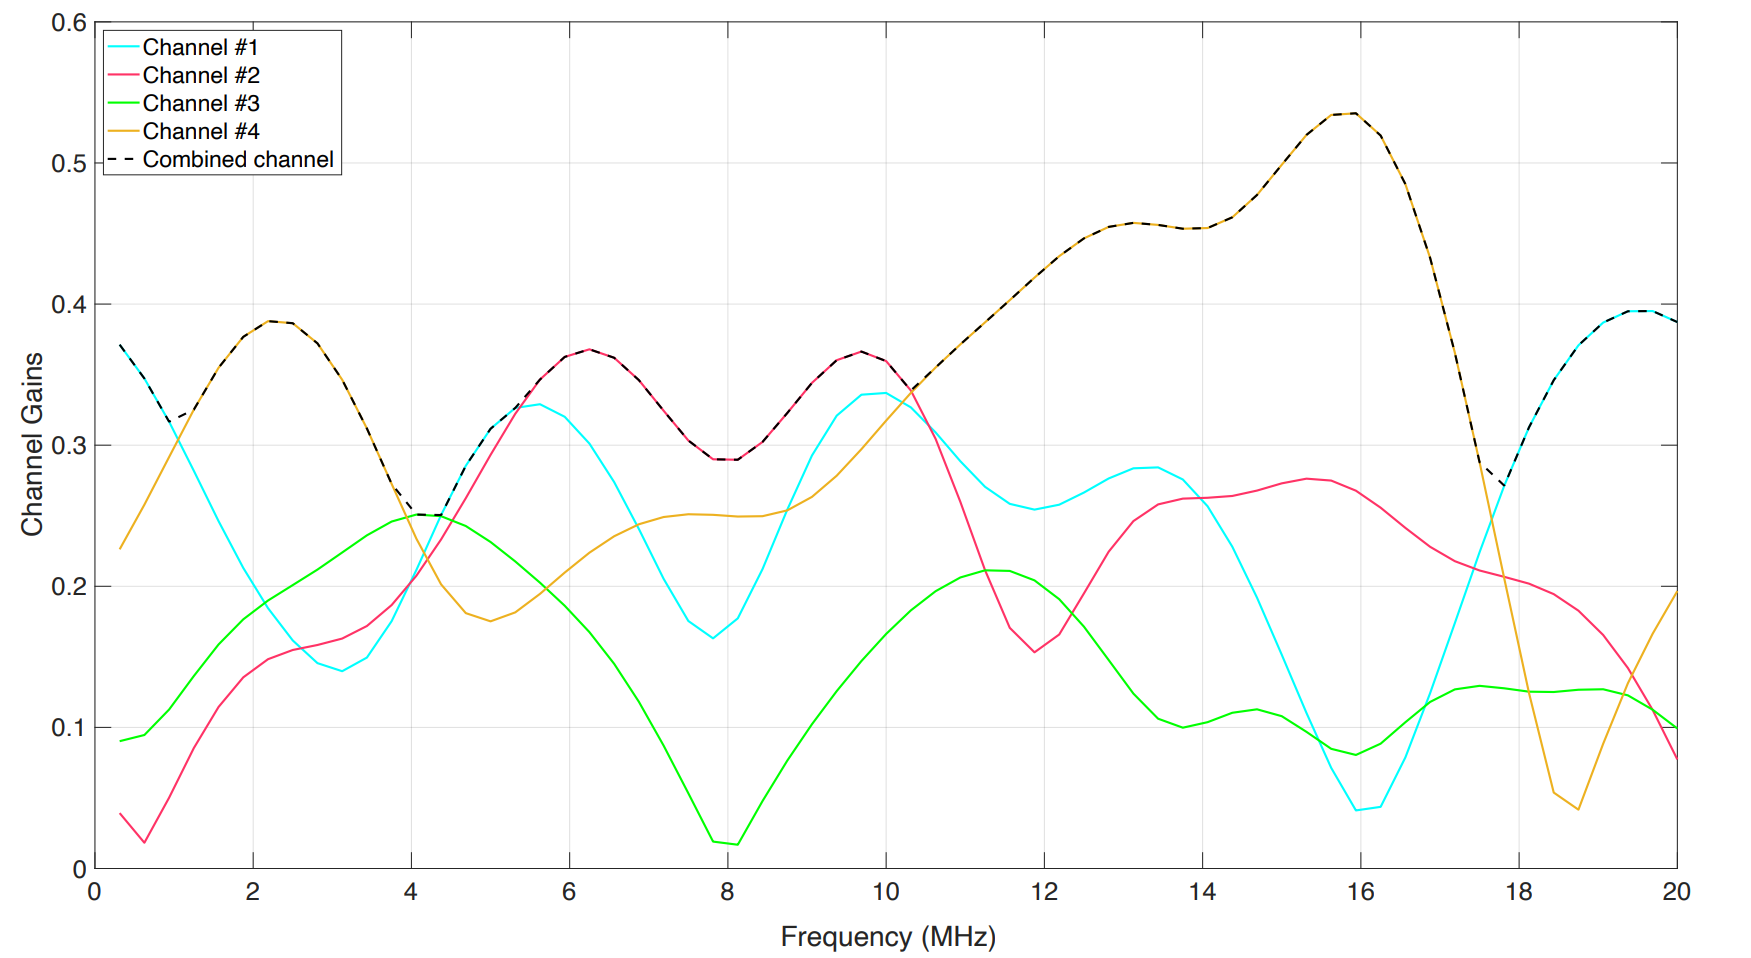
\includegraphics[width=0.675\textwidth]{imgs/diversity_graph.jpg}
\end{figure}


Il fading rappresenta il principale problema nelle comunicazioni radio, sebbene modulazioni come OFDM siano in grado di ridurre l'effetto del multipath fading, tuttavia lo \textbf{slow flat Rayleigh fading} non può essere contrastato nello stesso modo.

\begin{itemize}
    \item \textbf{Slow fading}: coherence time $>$ symbol period (doppler spread)
    \item \textbf{Flat fading}: delay spread $<$ symbol period (multipath time delay spread)
    \item \textbf{Rayleigh fading}: l'attenuazione delle repliche ha una distribuzione di Rayleigh.
\end{itemize}

I metodo principali per ridurre gli effetti di un fading di tali tipologie sono le diversity techniques, ovvero lo sfruttamente di canali con caratteristiche differenti per trasmettere la stessa informazione, aumentando la probabilità che il ricevitore possa ricostruire correttamente il messaggio.
Le principali tecniche di diversity sono:
\begin{itemize}
    \item \textbf{Time diversity}: relative al coherence time. Sfruttano trasmmissioni in slot temporali separati utilizzado anche \textbf{coding} e \textbf{interleaving}. Slow fading channels potrebbero non garantire una diversity sufficiente. Il canale deve variare sufficientemente in maniera veloce.
    \item \textbf{Frequency diversity}: relative alla coherence bandwidth. Sfruttano tramissioni su bande differenti. I flat fading channels potrebbero non garantire una diversity sufficiente.
    \item \textbf{Spatial diversity}: relative alla coherence distance. Sfruttano path di propagazione differenti, as esempio antenne differenti.
\end{itemize}

\subsection*{Time diversity: interleaving and coding}
Il channel coding consiste nell'introdurre dei bit ridondanti insieme a quelli trasmessi per rilevare eventuali errori al ricevitore e migliorare la bit error probability.
La ridondanza è misurata come:
\[
    R = \frac{k}{n} < 1, \quad \begin{cases}
        k \text{ bit contenenti informazione} \\
        n \text{ bit in uscita dall'encoder, contenenti informazione più ridondanza} \\
        n - k \text{ bit di ridondanza}
    \end{cases}
\]

Le operazioni effettuate sfruttano le proprietà matematiche del Galois Field GF(2), su cui sono definite somma (xor) e moltiplicazione (and) per due elementi $\{0, 1\}$.

\begin{figure}[ht]
    \centering
    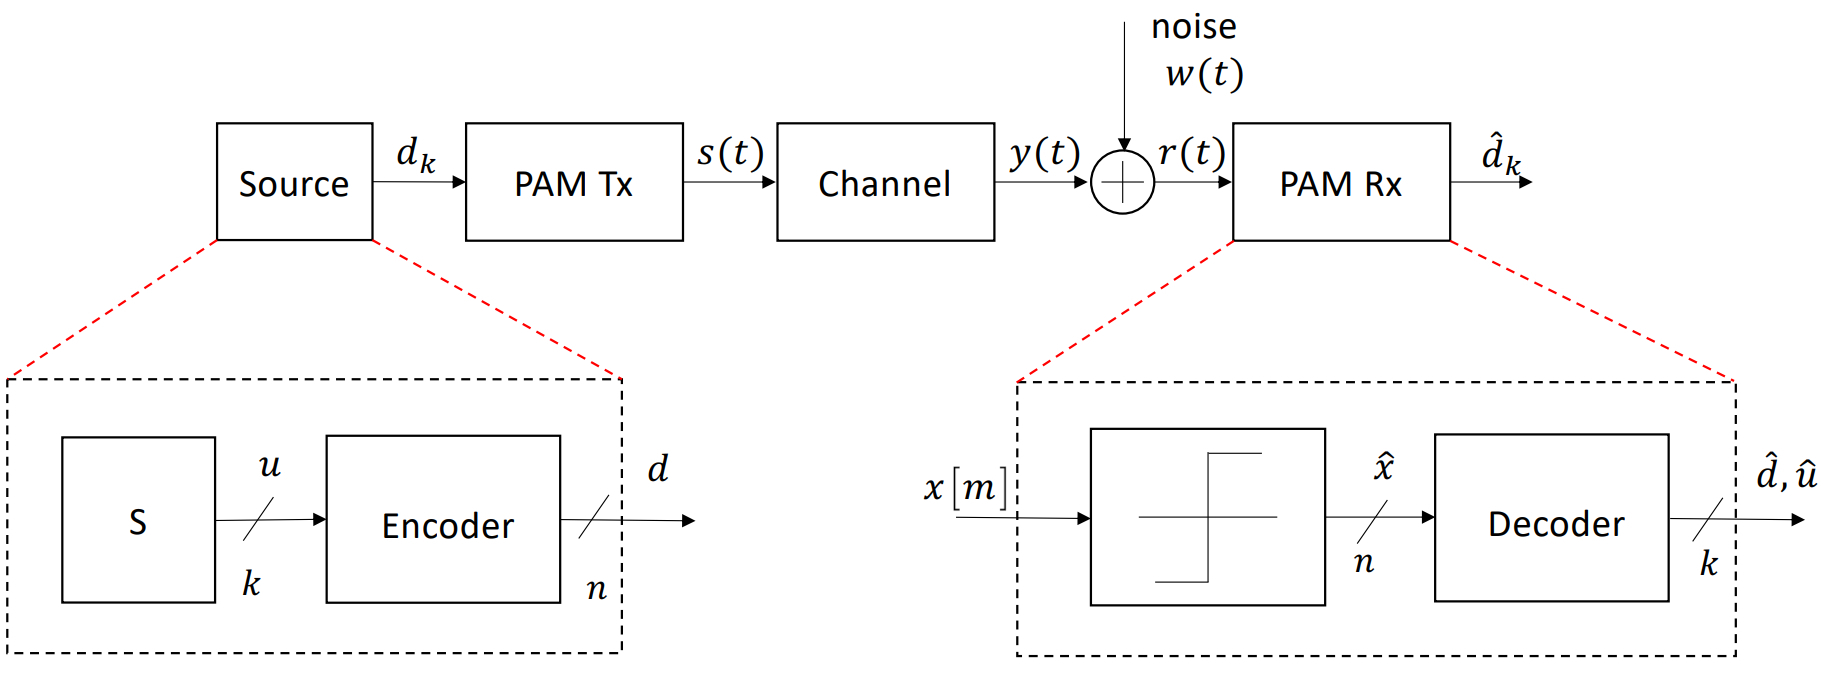
\includegraphics[width=0.675\textwidth]{imgs/encoder_decoder.jpg}
\end{figure}

Sorgente e destinazione introducono \textbf{encoder} e \textbf{decoder} per la gestione dei bit di ridondanza, si può utilizzare lo schema:


\begin{center}
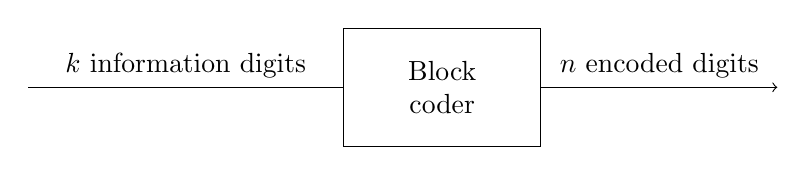
\begin{tikzpicture} [align=center]
    % Draw the block
    
    \node[draw, rectangle, minimum width=2.5cm, minimum height=1.5cm] (block) {Block \\ coder};
    
    % Draw the input arrow
    \draw[-] (block.west) -- ++(-4,0) node[midway, above] {$k$ information digits};
    
    % Draw the output arrow
    \draw[->] (block.east) -- ++(3,0) node[midway, above] {$n$ encoded digits};
\end{tikzpicture}
\end{center}


\begin{center}
    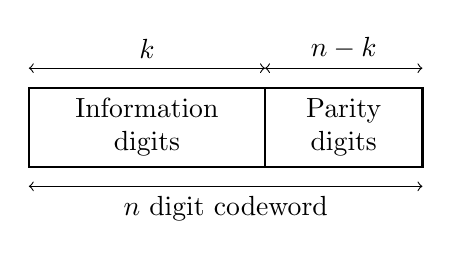
\begin{tikzpicture}[align=center]
    % Draw the main rectangle
    \draw[thick] (0,0) rectangle (5,1);
    
    % Draw the dividing line
    \draw[thick] (3,0) -- (3,1);
    
    % Labels inside the rectangles
    \node at (1.5,0.5) {Information\\digits};
    \node at (4,0.5) {Parity\\digits};
    
    % Arrows and labels
    \draw[<->] (0,1.25) -- (3,1.25) node[midway, above] {$k$};
    \draw[<->] (3,1.25) -- (5,1.25) node[midway, above] {$n-k$};
    \draw[<->] (0,-0.25) -- (5,-0.25) node[midway, below] {$n$ digit codeword};
\end{tikzpicture}

\end{center}

In questo schema l'intero sistema è visto come una componente che aggiunge un errore al messaggio trasmesso.

\paragraph*{Block code}
Si tratta della tipologia più semplice di coding in cui la coded word tramessa è composta da $n-k$ bit di parità.
L'operazione è rappresentabile come operazione di moltiplicazione fra un vettore (word da trasmettere) e una matrice (\textbf{generator matrix}, definisce il tipo di operazione).

\[
    \mathbf{d} = \mathbf{uG}, \quad \begin{cases}
        \mathbf{d} \text{ coded word} \quad d \in GF(2)^{1 \times n} \\
        \mathbf{u} \text{ word da trasmettere} \quad u \in GF(2)^{1 \times k} \\
        \mathbf{G} \text{ generator matrix} \quad G \in GF(2)^{k \times n}
    \end{cases}
\]

In generale le prime $k$ colonne della matrice $G$ equiavalgono a $I_k$ (matrice identità $k \times k$) e le restanti $n-k$ colonne sono i bit di ridondanza.
In totale si possono ottenere $2^k$ codeword differenti (uscita dell'encoder).
Si parla di coding sistematico quando i bit di informazione sono semplicemente copiati.

\paragraph*{Error detection}

\begin{center}   
    \begin{tikzpicture}
        % Nodes for the transmitter side
        \node[draw, rectangle, minimum width=1.5cm, minimum height=0.65cm] (T1) at (0,4) {Data 1};
        \node[draw, rectangle, minimum width=1.5cm, minimum height=0.65cm] (T2) at (3,4) {Data 2};
        \node[draw, rectangle, minimum width=1.5cm, minimum height=0.65cm] (T3) at (6,4) {Data 2};
        % create a node containing a red cross
        %\node[draw, cross out, red, thick, minimum size=1cm] (cross) at (4,3) {};
        % create a rotate of 45 degrees
        \node[draw, cross out, red, thick, minimum size=0.5cm, rotate=45] (cross) at (4,3) {};
        % Nodes for the receiver side
        \node[draw, rectangle, minimum width=1.5cm, minimum height=0.65cm] (R1) at (2,2) {Data 1};
        \node[draw, rectangle, minimum width=1.5cm, minimum height=0.65cm] (R2) at (5,2) {Data 2};
        \node[draw, rectangle, minimum width=1.5cm, minimum height=0.65cm] (R3) at (8,2) {Data 2};

        % Arrows for data transmission
        \draw[->, thick] (T1) -- (R1);
        \draw[->, thick] (R1) -- (T2) node[midway, above, sloped] {ACK};
        \draw[->, thick] (T2) -- (R2);
        \draw[->, thick] (R2) -- (T3) node[midway, above, sloped, red] {NACK};
        \draw[->, thick] (T3) -- (R3);

        % Arrow for time
        \draw[<->, dashed] (4.75,1.25) -- (7.75,1.25) node[midway, below] {$T_{ARQ} > T_c$};

        % Vertical lines for transmission boundaries
        \draw[dashed] (4.675,0.5) -- (4.675,3.5);
        \draw[dashed] (7.675,0.5) -- (7.675,3.5);
        
        % Labels for transmissions
        \node at (4.675,0) {1\textsuperscript{st} transmission};
        \node at (7.675,0) {2\textsuperscript{nd} transmission};
        
        % Labels for Transmitter and Receiver
        \node[] at (-2,4) {Transmitter};
        \node[] at (-2,2) {Receiver};
    \end{tikzpicture}
\end{center}



Le tecniche di error detection consistono nel confrontare i bit di ridondanza ricevuti con i bit di ridondanza calcolati utilizzando le word ricevute. Se il confronto ha successo si assume che la trasmissione non abbia introdotto errori, altrimenti si rileva un errore nella trasmissione.
In casi di errore il ricevitore può richiedere una nuova trasmission, adottando lo schema \textbf{ARQ} (Automatic Repeat reQuest). In tale schema ad ogni ricezione si risponde con un ACK o un NACK, in base al risultato del confronto. In caso di NACK si procede con una nuova trasmissione. 
Si tratta di una tecnica di time diversity, in quanto la ritrasmissione avviende dopo $T_{ARQ}$, un intervallo temporale superiore al coherence time del canale ($T_{ARQ} > T_c$).
Alcuni ricevitori sono in grado di cambiare i due messaggi ricevuto, incrementando la probabilità di ricostruire l'informazione trasmessa.
Una semplice tecnica di error detection è il \textbf{parity check code}, in cui si aggiunge un bit di parità alla fine della word di 7 bit da trasmettere. Se il numero di bit a 1 è pari, il bit di parità è 0, altrimenti è 1.

\[
    \begin{cases}
        k = 7 \\
        n = 8 
    \end{cases}
    \Rightarrow R = \frac{7}{8},
    \quad \mathbf{G} = \left[I_7, 1_7\right] = 
    \begin{bmatrix}
        1 & 0 & 0 & 0 & 0 & 0 & 0 & 1 \\
        0 & 1 & 0 & 0 & 0 & 0 & 0 & 1 \\
        0 & 0 & 1 & 0 & 0 & 0 & 0 & 1 \\
        0 & 0 & 0 & 1 & 0 & 0 & 0 & 1 \\
        0 & 0 & 0 & 0 & 1 & 0 & 0 & 1 \\
        0 & 0 & 0 & 0 & 0 & 1 & 0 & 1 \\
        0 & 0 & 0 & 0 & 0 & 0 & 1 & 1 \\
    \end{bmatrix}
    \Rightarrow u_7 = \sum_{i=0}^{6} u_i
\]
Il parity bit è calcolato sommando tutti i bit delle word usando l'algebra in GF(2).
Sebbene sia molto semplice questa tecnica, non può essere sempre efficace in quanto può riconoscere unicamente un numero di errori dispari, mentre in caso di numero di errori pari si avrà un bilanciamente degli 1 ed il confronto avrà successo.

\paragraph*{Error correction}
Le tecniche di error correction sono utilizzate per rilevare e correggere errori di trasmissione, senza necessità di richiedere una nuova trasmissione.
Dato un canale si definisce \textbf{capacità} il massimo rate a cui è possibile trasmettere:
\[
    C = B \log_2(1 + \text{SNR}) \quad \text{bit/s}
\]

Ogni trasmissione con rate $R < C$ ed $\epsilon$ arbitratio è possibile determinare un error correction code per cui $P_e < \epsilon$.
Una semplice tecnica di error correction è il \textbf{repetition code}, in cui la word è ripetuta 3 volte. Per stabilire quale sia il bit corretto in casi si incongruenza si adotta una strategia maggioritaria.


\[
    \begin{cases}
        k = 1 \\
        n = 3 
    \end{cases}
    \Rightarrow R = \frac{1}{3},
    \quad \mathbf{G} =
    \begin{bmatrix}
        1 & 1 & 1
    \end{bmatrix}
    \quad 
    \begin{cases}
        u = \begin{bmatrix}0\end{bmatrix} \Rightarrow d = \begin{bmatrix}0 & 0 & 0\end{bmatrix} \\
        \\
        u = \begin{bmatrix}1\end{bmatrix} \Rightarrow d = \begin{bmatrix}1 & 1 & 1\end{bmatrix}
    \end{cases}
\]


Questa tecnica è in grado di correggere un unico errore, tuttavia se utilizzato come error detection può rilevare fino a due errori.
La distanza tra due codeword è calcolata come numero di bit differenti fra le due stringhe, detta anche \textbf{Hamming distance}. Il decoder selezione le word con minima distanza rispetto a quella ricevuta.

\[
    \hat{d} = \text{argmin}_d \left\{\text{distance}(d, \hat{x})\right\}
\]

Dove $\hat{d}$ è la word in uscita dal decoder, $d$ è una word possibile e $\hat{x}$ è la word ricevuta
Gli errori possono far scegliere al decoder la word sbagliata, la capacità di error correction di un block code è tanto maggiore quanto maggiore è la Hamming distance tra le codeword generabili. La bontà del block code è misurabile con la minima distanza tra codewords $d_{min}$.
\[
    d_{min} - 1 \quad \text{Numero massimo di errori rilevabili}
\]

\[
    \left\lfloor \frac{d_{min} - 1}{2} \right\rfloor \quad \text{Numero massimo di errori correggibili}
\]
Maggiore è la distanza di Hamming, maggiore è la ridondanza da aggiungere.
Fissata $R=\frac{k}{n}$, $d_{min}$ sarà più grande al crescere di $k$ e $n$, tuttavia si complica anche il sistema.
\section*{Convolutional code}

I codici convoluzionali, al contrario dei block code, non sono sistematici, si trasmettono infatti solo i bit di parità.
L'encoder utilizza una sliding window per generare $n>1$ bit di parità, combinando vari sottoinsiemi di bit nel campo GF(2), realizzando una sorta di convoluzione.
L'encoder si comporta come $n$ filtri lineari in paraellelo, i parametri che lo costituiscono sono:
\begin{itemize}
    \item $n$: bit generati
    \item $k$: bit di informazione (si considererà sempre $k=1$)
    \item $L$: lunghezza del vincolo, ovvero il numero di parole di input di $k$ bit che concorrono alla generazione degli $n$ bit dvincolo, ovvero il numero di parole di input di $k$ bit che concorrono alla generazione degli $n$ bit di output. Nel caso di $k=1$ sarà la lunghezza dei bit che concorrono alla generazione del codice.
\end{itemize}

La dimensione della finestra corrisponde a $L-K$, quindi si considererà $L-1$. Il codice generato, oltre alla word, è anche funzione dei bit di input precedenti. Ogni bit generato è ottenuto dalla convoluzione in GF(2) con una risposta impulsiva rappresentata da un diverso generatore $g$, di dimensione $kL$.
I bit in uscita sono quindi un flusso continuo e non organizzati in blocchi.

Trattandosi di sistemi con memoria, l'encoder può essere rappresentato come una macchina a stati finiti.
L'output dell'encoder dipende dal bit in input e dalla stato corrente.
L'evoluzione temporale dell'encoder può essere catturata dal \textbf{trellis diagram}, in cui si ha l'evoluzione degli stati in funzione del tempo.
Ogni sequenza, con la corrispondente encoded word, può essere rappresentata come un cammino nel trellis diagram.
Una trasmissione di $N$ codewords implica la trasmissione di $n \cdot N$ bits, ottenuti dalla codifica di $k \cdot N$ input word.
Poiché ogni codeword è funzione anche di $L-1$ input word precedenti, la sequenza può essere codificata considerandola solo nella sua interezza. 
Il decoder dovrà scegliere la sequenza più "vicina" rispetto a quella ricevuta tra tutte le possibili sequenza, ovvero $2^{k \cdot N}$
\[
    \hat{d} = \text{argmin}_d \left\{\text{distance}(d, \hat{x})\right\}
\]
Dove d è una possibile sequenza, $\hat{x}$ è la sequenza ricevuta e $\hat{d}$ è la sequenza in uscita dal decoder.
L'utilizzo nella pratica di codici convoluzionali è stata resa possibile solo dall'introduzione dell'algoritmo di Viterbi, in grado di applicare una decodifica con complessità lineare e non più esponenziale.

\paragraph*{Algoritmo di Viterbi}
L'obiettivo è trovare la sequenza con distanza minima rispetto a quella ricevuta:

\[
    \hat{d} = \text{argmin}_d \left( d_H \left(\tilde{d}, \hat{x}\right) \right)
\]
Le possibili sequenza $\tilde{d}$ sono viste come sequene di $N$ blocchi, ciascuna composta da 
$n$ bit, ovver i bit prodotti a partire dai $k$ bit di informaione in ingresso all'encoder.


\[
    d_H\left(\tilde{d}, \hat{x}\right) = \sum_{j=1}^{N} d_H\left(\tilde{d}_j, \hat{x}_j\right)
\]

Dove $d_H$ è la distanza di Hamming tra due sequenze di bit, $\tilde{d}_j$ è la $j$-esima codeword possibile e $\hat{x}_j$ è la $j$-esima codeword ricevuta.
Ogni sequenza $\tilde{d}$ corrisponde ad una seuqenza di stati $\tilde{S}_0, \ldots, \tilde{S}_N$ nel diagramma a trabocco, ovvero a un determinato path. La $j$-esima uscita dell'encoder, $\tilde{d}_j$, dipende dalla transizione tra gli stati $\tilde{S}_{j-1}$ e $\tilde{S}_j$.
.
.
.
.

% insert python code hello world hre
La distanza di Hamming può essere calcolata in Python come:
\begin{minted}{python3}
def hamming_distance(a: int, b: int) -> int:
    return bin(a ^ b).count('1')
\end{minted}


Dal Trellis diagram possiamo dedurre la funzione di transizione come:
\begin{minted}{python3}

def state_machine(state: int, input_bit: bool) -> Tuple[int, int]:
    match state:
        case 0b01:
            return (0b11, 0b00) if not input_bit else (0b00, 0b10)
        case 0b10:
            return (0b10, 0b01) if not input_bit else (0b01, 0b11)
        case 0b11:
            return (0b01, 0b01) if not input_bit else (0b10, 0b11)
        case 0b00:
            return (0b00, 0b00) if not input_bit else (0b11, 0b10)
        case _:
            raise ValueError("Invalid state")

\end{minted}
Per quanto riguarda invece l'algoritmo di Viterbi, esso può essere definito per sommi capi come:

\begin{minted}{python3}
def viterbi_algorithm(sequence: List[bool]) -> List[bool]:
    chunks: List[int] = bit_pairs_to_integers(sequence)
    matrix: List[List[Optional[ViterbiCell]]] = populate_matrix(chunks)
    final_state = get_last_state(matrix)
    return get_decoded_sequence(matrix, final_state)
\end{minted}

La funzione \textit{populate\_matrix} riempie una matrice con celle di Viterbi aggiornando distanze globali e stati successivi per ogni colonna di input.

\begin{minted}{python3}
def populate_matrix(chunks: List[int]) -> List[List[Optional[ViterbiCell]]]:
    matrix: List[List[Optional[ViterbiCell]]] = empty_matrix(rows=4, cols=len(chunks) + 1)
    matrix[0][0] = ViterbiCell(prev_state=0, global_distance=0, input_bit=False)

    for col in range(len(chunks)):
        for row in range(4):
            current_cell = matrix[row][col]
            if current_cell is None:
                continue
            for input_bit in [False, True]:
                output, next_state = state_machine(row, input_bit)
                new_distance = current_cell.global_distance + hamming_distance(output, chunks[col])
                next_cell = matrix[next_state][col + 1]
                if next_cell is None or next_cell.global_distance > new_distance:
                    matrix[next_state][col + 1] = ViterbiCell(
                        row, new_distance, input_bit
                    )
    return matrix
\end{minted}
La funzione \textit{get\_last\_state} trova lo stato finale con la distanza globale minima nell'ultima colonna della matrice.
\begin{minted}{python3}
def get_last_state(matrix: List[List[Optional[ViterbiCell]]]) -> int:
    min_distance = float('inf')
    final_state = None
    for i in range(4):
        last_row_cell = matrix[i][-1]
        if last_row_cell and last_row_cell.global_distance < min_distance:
            min_distance = last_row_cell.global_distance
            final_state = i
    return final_state
\end{minted}
La funzione \textit{get\_decoded\_sequence} ricostruisce la sequenza decodificata risalendo dalla matrice a partire dallo stato finale.
\begin{minted}{python3}
def get_decoded_sequence(matrix: List[List[Optional[ViterbiCell]]], final_state: int) -> List[bool]:
    sequence_length = len(matrix[0]) - 1
    decoded_sequence: List[bool] = [False] * sequence_length
    
    current_state = final_state
    for i in range(sequence_length - 1, -1, -1):
        cell = matrix[current_state][i + 1]
        decoded_sequence[i] = cell.input_bit
        current_state = cell.prev_state

    return decoded_sequence
\end{minted}


Come esempio consideriamo di voler trasmettere la sequenza di bit $010000$, l'encoder emetterà quindi la sequenza $00 \ 11 \ 10 \ 11 \ 00 \ 00$. Supponendo che il decoder riceva la sequenza $00 \ 10 \ 10 \ 11 \ 00 \ 00$, l'algoritmo di Viterbi sarà in grado di correggere l'errore e restituire la sequenza corretta $010000$.




\begin{center}
    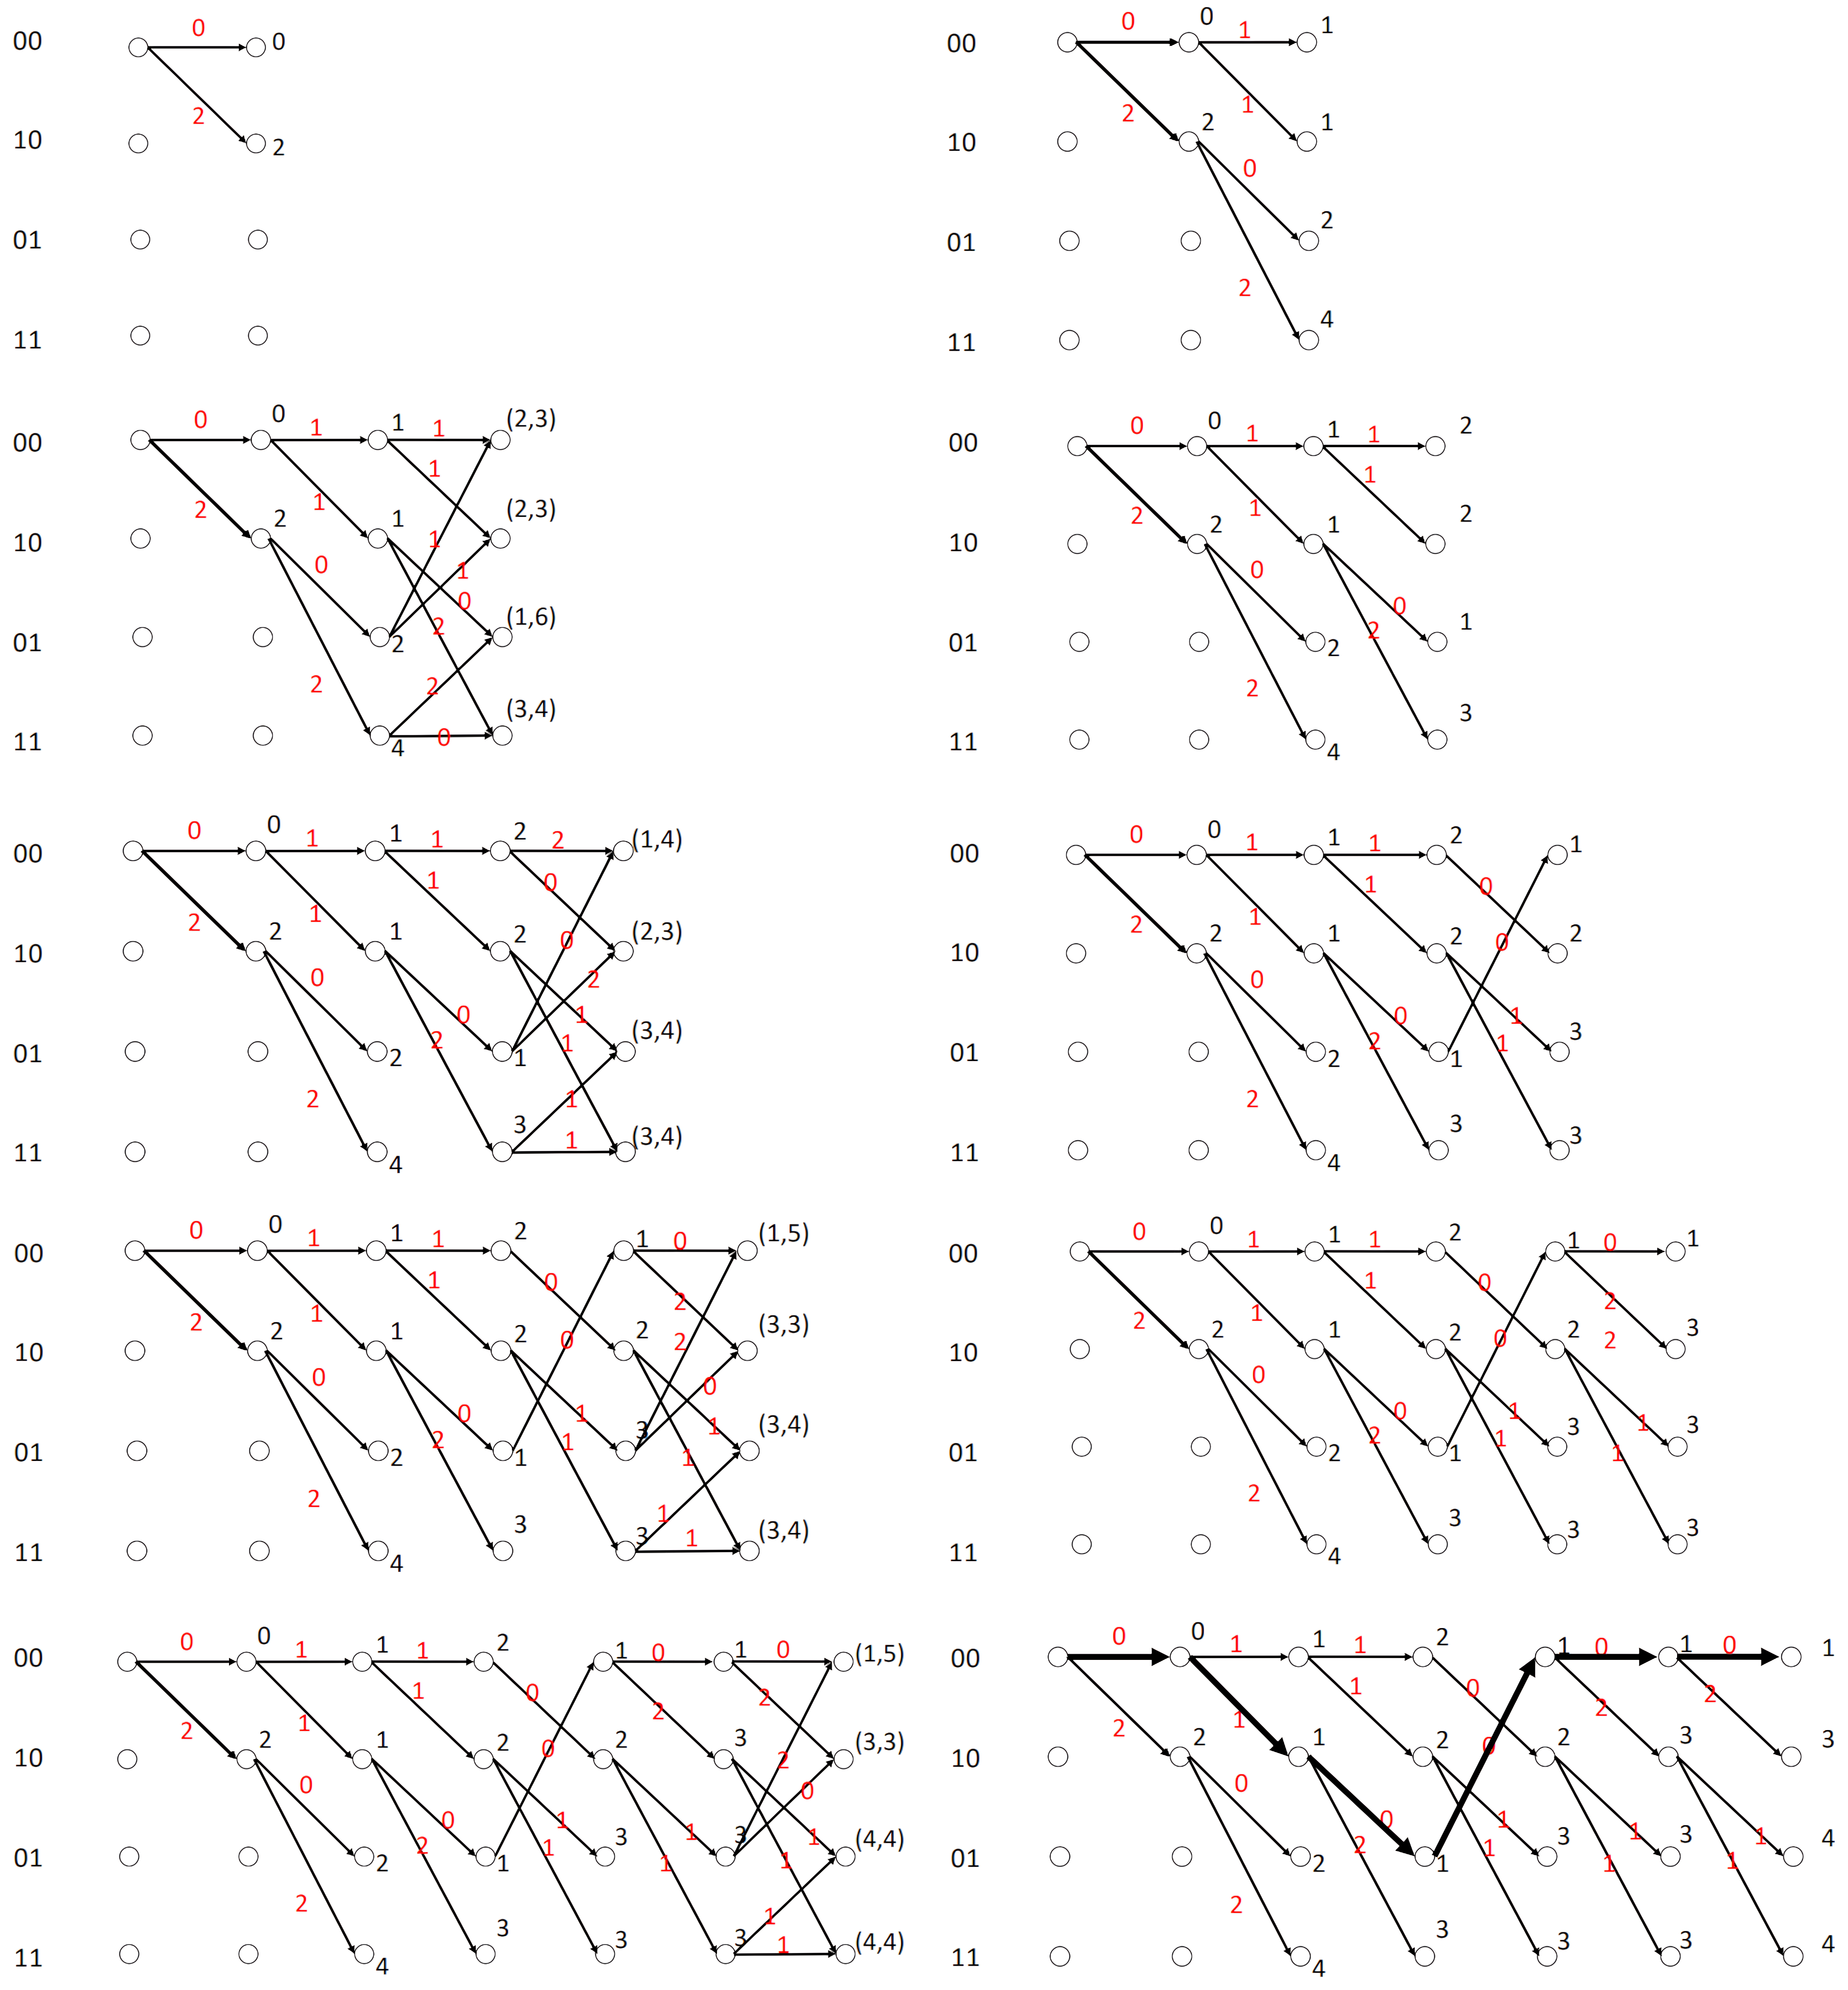
\includegraphics[width=1\textwidth]{imgs/viterbi_example.png}
\end{center}


Ovvero eseguendo l'algoritmo in Python si ottiene la seguente rappresentazione in memoria, stampando i campi \textit{prev\_state}, \textit{global\_distance} e \textit{input\_bit} per ogni cella della matrice:


\begin{table}[h!]

\resizebox{\textwidth}{!}{
    \centering
    \begin{tabular}{|c|c|c|c|c|c|c|c|}
    \hline
    State & Column 1 & Column 2 & Column 3 & Column 4 & Column 5 & Column 6 & Column 7 \\
    \hline
    Row 0b00 & 0b00, 0, 0 & \textbf{0b00, 0, \textcolor{red}{0}} & 0b00, 1, 0 & 0b00, 2, 0 & \textbf{0b01, 1, \textcolor{red}{0}} & \textbf{0b00, 1, \textcolor{red}{0}} & \textbf{0b00, 1, \textcolor{red}{0}} \\
    \hline
    Row 0b10 & None & 0b00, 2, 1 & \textbf{0b00, 1, \textcolor{red}{1}} & 0b00, 2, 1 & 0b00, 2, 1 & 0b00, 3, 1 & 0b00, 3, 1 \\
    \hline
    Row 0b01 & None & None & 0b10, 2, 0 & \textbf{0b10, 1, \textcolor{red}{0}} & 0b10, 3, 0 & 0b10, 3, 0 & 0b10, 4, 0 \\
    \hline
    Row 0b11 & None & None & 0b10, 4, 1 & 0b10, 3, 1 & 0b10, 3, 1 & 0b10, 3, 1 & 0b10, 4, 1 \\
    \hline
    \end{tabular} 
        
    }
    \end{table}

\section*{Interleaving}



\begin{center}
    \resizebox{\textwidth}{!}{
    \begin{tikzpicture}[node distance=1.5cm, auto, >=Stealth, minimum height=1cm, minimum width=1.5cm]
        % Nodes
        \node[draw, rectangle] (S) {S};
        \node[draw, rectangle, right=of S] (Encoder) {Encoder};
        \node[draw, rectangle, right=of Encoder] (Interleaver) {Interleaver};
        \node[draw, rectangle, right=of Interleaver] (Channel) {Channel};
        \node[draw, rectangle, right=of Channel] (Deinterleaver) {Deinterleaver};
        \node[draw, rectangle, right=of Deinterleaver] (Decoder) {Decoder};
        \node[right=of Decoder, inner sep=0pt, minimum size=0pt] (Uhat) {};

        % Connections
        \draw[->] (S) -- node {$u$} (Encoder);
        \draw[->] (Encoder) -- (Interleaver);
        \draw[->] (Interleaver) -- node {$d$} (Channel);
        \draw[->] (Channel) -- node {$x$} (Deinterleaver);
        \draw[->] (Deinterleaver) -- (Decoder);
        \draw[->] (Decoder) -- node {$\hat{u}$} (Uhat);


        % Dashed boxes
        \draw[dashed] ($(S.north west)+(-0.5,0.5)$) rectangle ($(Interleaver.south east)+(0.5,-0.5)$);
        \draw[dashed] ($(Deinterleaver.north west)+(-0.5,0.5)$) rectangle ($(Decoder.south east)+(0.5,-0.5)$);
    \end{tikzpicture}
}
\end{center}
\begin{center}
    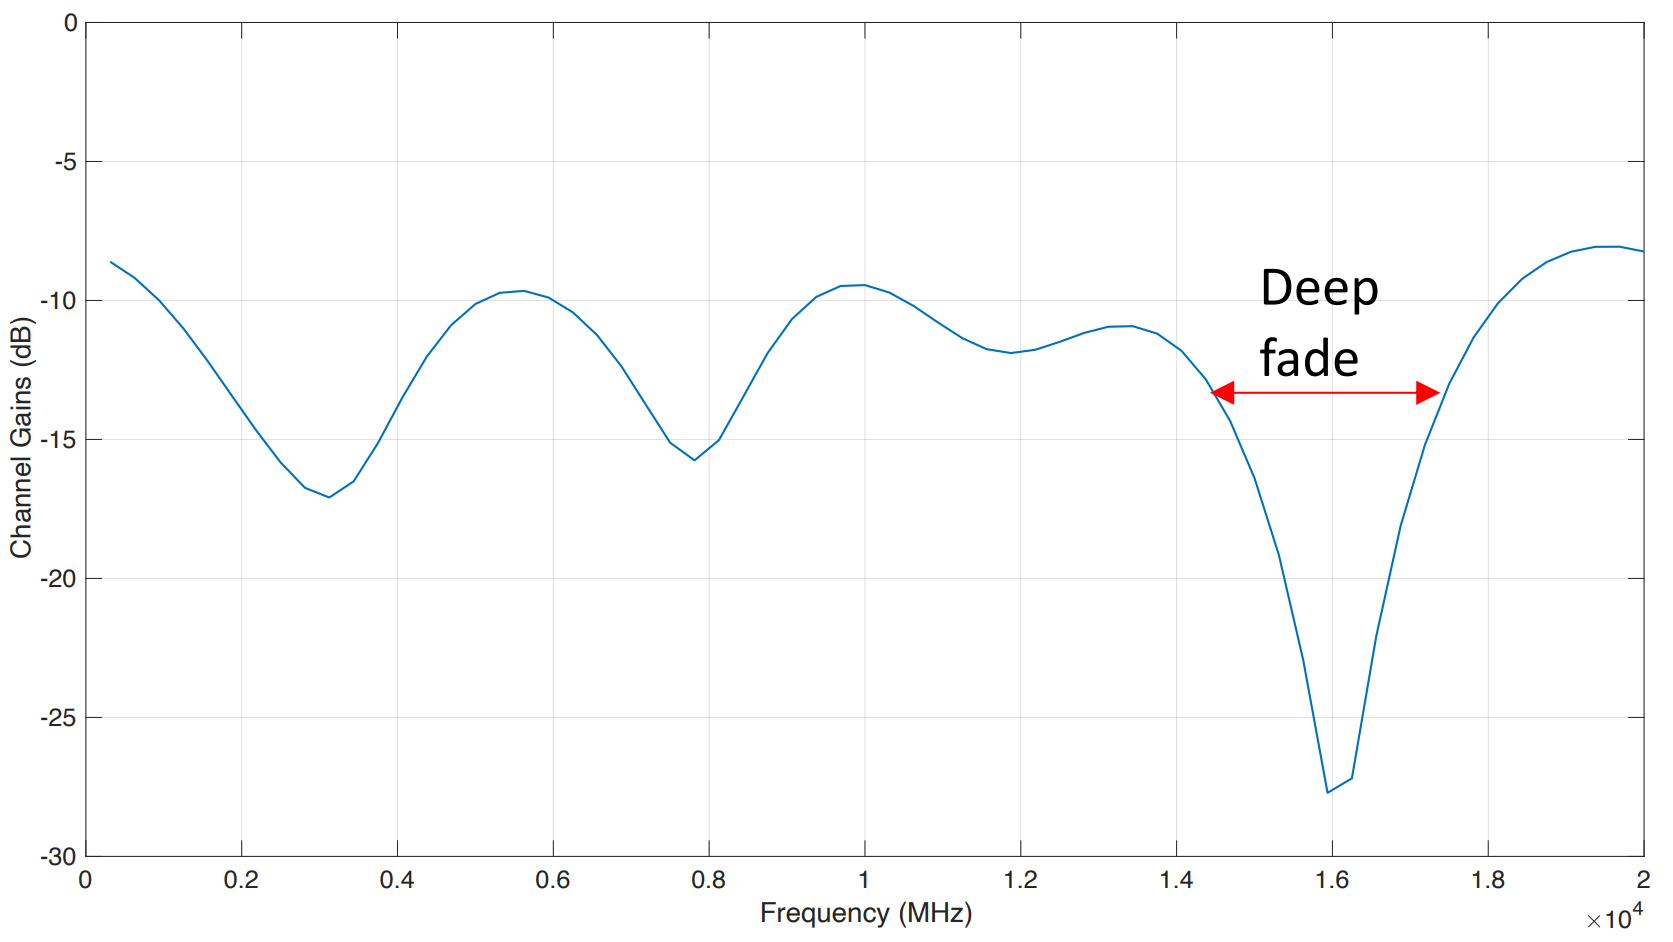
\includegraphics[width=0.5\textwidth]{imgs/deep_fade.png}
\end{center}

I codici convoluzionali risultano adatti per canali memoryless con errori randomici, uniformamente distribuiti ed incorrelati. 
Tuttavia un canale fading è tipicamente suggetto a \textbf{bursty errors}, ovvero genera un gruppo di errori consecutivi nel tempo e/o in frequenza. 
Quando il canale è in \textbf{deep fade} ci sono delle dipendenze statistiche tra errori consecutivi.
L'idea dell'interleaving consiste nel far sembrare il canale memoryless dal punto di vista del decoder, de-correlando gli errori provocati dal canale, semplicemente rimescolando i bit prodotti dell'encoder prima di effettuare la trasmissione.
Lato ricevitore prima del decoder si effettuare un'operazione di de-interleaving per ripristinare l'ordine originale.
Il costo delle operazioni di (de-)interleaving è pagato in termini di latenza in quanto sia lato ricevitore che lato trasmettitore è necessario avere un intero blocco di dati prima di poter effettuare le operazioni. 
Esiste un trade-off tra latenza e decorrelazione ottenibile, basata sulla profondità $k$ dell'interleaver, ovvero la dimensione del blocco sul quale si effettua l'operazione di rimescolamento.

Per esempio disponendo una sequenza dentro una matrice, possiamo ottenere un interleaver considerando la trasposta:
\begin{table}[h!]
    \centering
    \begin{tabular}{c}
    
    \begin{tabular}{|c|c|c|c|}
    \hline
    A & B & C & D \\ \hline
    E & F & G & H \\ \hline
    I & J & K & L \\ \hline
    M & N & O & P \\ \hline
    \end{tabular}
    
    \quad $\rightarrow$ \quad
    
    \begin{tabular}{|c|c|c|c|}
    \hline
    A & E & I & M \\ \hline
    B & F & J & N \\ \hline
    C & G & K & O \\ \hline
    D & H & L & P \\ \hline
    \end{tabular}
    
    \end{tabular}
\end{table}
   

\begin{center}
    \resizebox{\textwidth}{!}{
    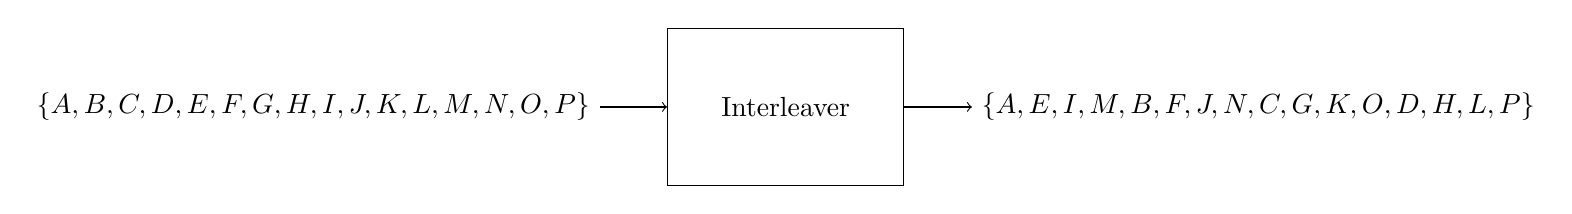
\begin{tikzpicture}
        \node (input) at (0,0) {$\{A,B,C,D,E,F,G,H,I,J,K,L,M,N,O,P\}$};
        \node[draw, minimum height=2cm, minimum width=3cm, align=center] (interleaver) at (6,0) {Interleaver};
        \node (output) at (12,0) {$\{A,E,I,M,B,F,J,N,C,G,K,O,D,H,L,P\}$};

        \draw[->] (input) -- (interleaver);
        \draw[->] (interleaver) -- (output);
    \end{tikzpicture}
    }
\end{center}



\paragraph*{Turbo code e LDPC (Low Density Parity Check)}
Nella formula della capacità del canale di Shannon\footnote{$C=B\log_2(1+\text{SNR}) \si{b/s}$} il rate $R = \frac{k}{n}$ prevede sia $k$ che $n$ tendenti all'infinito, tuttavia la lunghezza del codice nei sistemi reali è finito, quindi ciò che si ottiene è una performance lontana da quella teorica.
Negli anni sono stati introdotti nuovi codici, sempre più efficienti, tra cui turbo code e LDPC, i quali si avvicinano al limite teorico imposto dalla formula di Shannon.


Più nel dettaglio abbiamo lato trasmettitore da eseguire i seguenti passi:

\begin{center}
    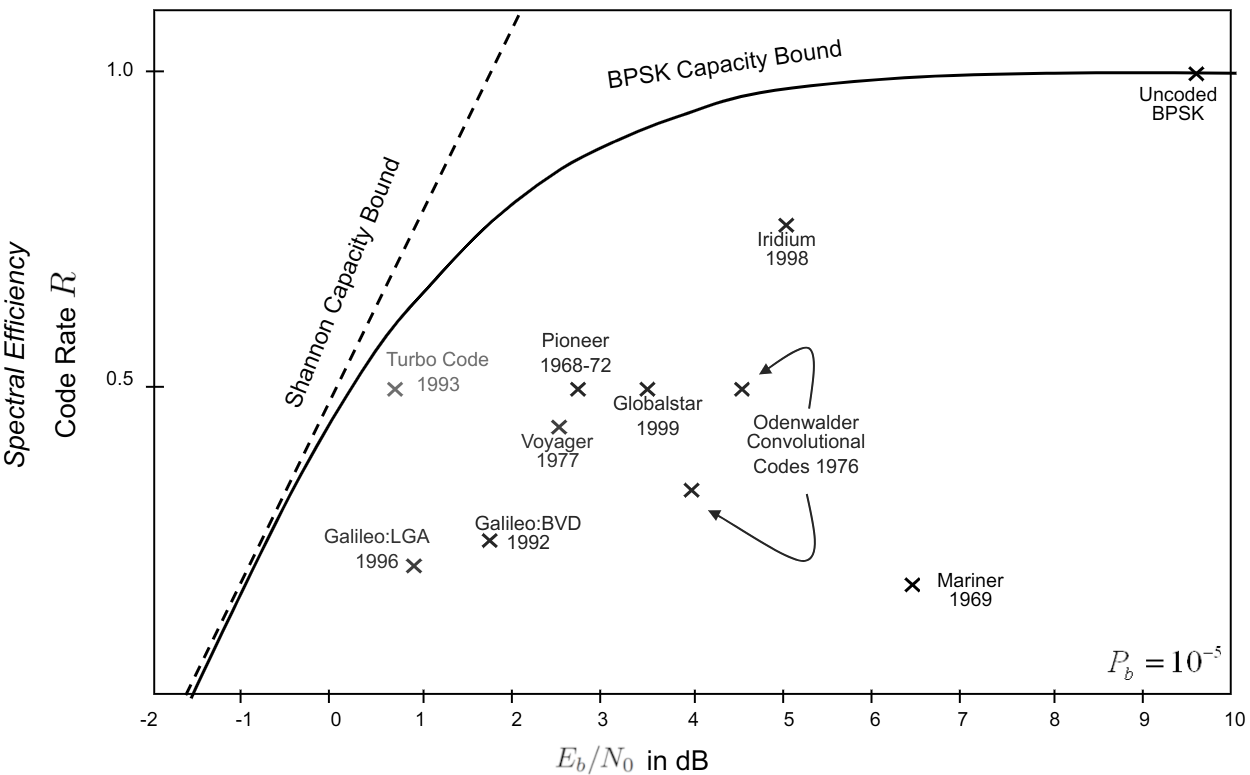
\includegraphics[width=0.5\textwidth]{imgs/codes_and_shannon_bound.png}
\end{center}
\paragraph*{Turbo code (error correction)}

Si tratta di un convolutional code in cui sono utilizzati due encoder in parallelo in grado di generare due sequenze indipendenti, migliorando il processo di decoding grazie alla ridondanza ottenuta e alla diversity, ottenuta dalla presenza di uno stream di dati differente.
Il sistema è composto da tre sequenze di cui due codificate e una inalterata. L'utilizzo dell'interleaver permette di estendere artificialmente la lunghezza della sequenza, avvicinandosi alle ipotesi di Shannon. Inoltre l'interleaver permette di ottenere sequenze indipendenti. 
Il trasmettitore invia quindi tre sequenze, tra cui quella originaria, ottenendo un $R=\frac{1}{3}$. L'idea è che se il canale produce un errore le due sequenze prodotte in maniera differente possono essere unite  per correggere l'errore.
Per quanto riguarda il decoder si utilizzano due decoder in cascata, il primo prevede in ingresso i bit sistematici e la prima sequenza generanza senza interleaving. L'output prodotto invece di essere utilizzato come uscita del sistema è inviato ad un inteleaver, assieme ai bit sistematici. 
Le due sequenze dopo l'interleaving sono mandate in ingresso, assieme alla seconda sequenza di parità, al secondo decoder. L'uscita è infine inviata al deinterleaver. 
Completato il primo ciclo è possibile effettuarne altri, mandando nuovamente in ingresso al primo decoder l'uscita dell'interleaver. 
L'uscita dei decoder rappresenta una stima, sempre più accurata, della sequenza trasmessa. Il processo iterativo va avanti finché vi sono modifiche nei bit decifrati.
In generale se il SNR rispetta le condizioni di Shannon l'impiego di turbo codes permette di effettuare la correzione degli errori ed ottenere dei BER molto bassi, tuttavia il prezzo è ancora pagato in termini di latenza.






\begin{center}

    \begin{figure}[h!]
        \centering
        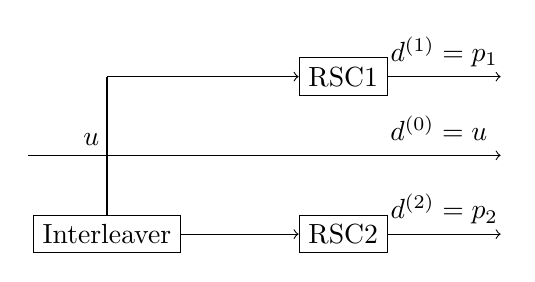
\begin{tikzpicture}
    
            % Draw blocks
            \node[draw, rectangle] (RSC1) at (3,2) {RSC1};
            % dummy node for alignment
            \node[inner sep=0pt, minimum size=0pt] (dummy) at (3,1) {};
            \node[draw, rectangle] (Interleaver) at (0,0) {Interleaver};
            \node[draw, rectangle] (RSC2) at (3,0) {RSC2};
            
            \draw[->] (0,2) -- (RSC1) node[midway, above] {};
            \draw[->] (RSC1) -- (5,2) node[midway, above] {$d^{(1)} = p_1$};
            \draw[->] (Interleaver) -- (RSC2);
            \draw[->] (RSC2) -- (5,0) node[midway, above]{$d^{(2)} = p_2$}; 
            \draw[->] (-1,1) -- (5,1) node[midway, above, xshift=63, yshift=2] {$d^{(0)} = u$};
            \draw[-] (Interleaver) -- (0, 2) node[midway, left] {}; 
            \node at (-0.2,1.2) {$u$};
            
        \end{tikzpicture}
        \caption{}
       
        \label{fig:turbo_encoder}
    \end{figure}
\end{center}
\begin{enumerate}
    \item I bit di informazione (e.g. $01101$) entrano nel trasmettitore e vengono copiati negli encoder RSC1 RSC2. Prima di entrare in RSC2, i bit di informazione vengono rimescolati dall'interleaver (e.g. $10011$).
    \item Ogni encoder genera una stringa di bit di correzione di errore (bit di parità) eseguendo una serie di calcoli sui bit di dati che riceve (e.g. rispettivamente, $10110$ e $11100$).
    \item I bit di informazione e le due stringhe di bit di parità sono combinati in un unico blocco e inviati sul canale, dove il rumore può causare errori nella trasmissione.
\end{enumerate}

Per quanto rigurda la ricezione, il processo è il seguente:

\begin{center}
    \begin{tikzpicture}[node distance=1.5cm, auto, >=Stealth, minimum height=1cm, minimum width=1.5cm]

        \node[draw, rectangle] (D1) at (3,0) {D1};
        \node[draw, rectangle] (I) at (6,0) {I};
        \node[draw, rectangle] (D2) at (9,0) {D2};
        \node[draw, rectangle] (InvI) at (6,2) {Inv(I)};

        \draw[->] (0,0) -- (2.25, 0) node[midway, above] {$\hat{p}_1$};
        \draw[->] (0,-0.875) -| (D1) node[midway, below] {$\hat{u}$};
        \draw[->] (0,-1.75) -| (I) node[midway, below] {$\hat{p}_2$};
        \draw[->] (3,-0.875) -| (5.675, -0.5) node[midway, below] {};
        \draw[->] (D1) -- (I) node[midway, above] {Le12};
        \draw[->] (I) -- (D2);
        \draw[->] (D2) |- (InvI) node[midway, right] {Le21};
        \draw[->] (InvI) -| (D1);
        % TODO: a cosa serve la seconda freccia?
        %\draw[->] (6.25, -0.5) -- ++(0,-0.875) -| (D2);
    \end{tikzpicture}
\end{center}



\begin{enumerate}
    \item Al segnale (campionato) viene associata una lista di interi (e.g. $[7, -5, 5, 2, -4; \ 6, 5, 7 -2, \textcolor{red}{-2}; \ 3, 8, 1, -5, -3]$, dove $\hat{p}_1$, $\hat{u}$ e $\hat{p}_2$ sono stati separati da un punto e virgola, mentre il rosso è idicata una predizione sbagliata), 
    i cui elementi indicano quanto è probabile che un bit sia 0 o 1. Ad esempio, -7 significa che il bit è quasi certamente un 0; +7 significa che è quasi certamente un 1. Notare che un errore è avvenuto nel quinto bit del blocco: originariamente un 1, ora ha un valore negativo, che suggerisce un 0 logico.
    \item Ogni decoder prende la lista contenente l'informazione con rumore e la rispettiva lista di parità e calcola quanto è sicuro di ciascun bit decodificato. I due decoder scambiano queste informazioni di confidenza ripetutamente e dopo un certo numero di iterazioni, tipicamente da quattro a dieci, iniziano ad essere d'accordo su tutti i bit decodificati. 
    \item I dati decodificati sono la somma della lista contenente l'informazione (con rumore, e.g. $[6, 5, 7 -2, \textcolor{red}{-2}]$) più le due liste finali contenti i valori di confidenza(e.g. $[-5, 3, 7, -6, 5]$ e $[-3, 4, 2, -4, 3]$). L'output ($[-14, 12, 16, -12, 6]$) viene convertito nuovamente in bit binari ($[0, 1, 1, 0, 1]$,  da cui si può notare che il quinto bit ora ha il valore corretto).
\end{enumerate}



\begin{center}
    
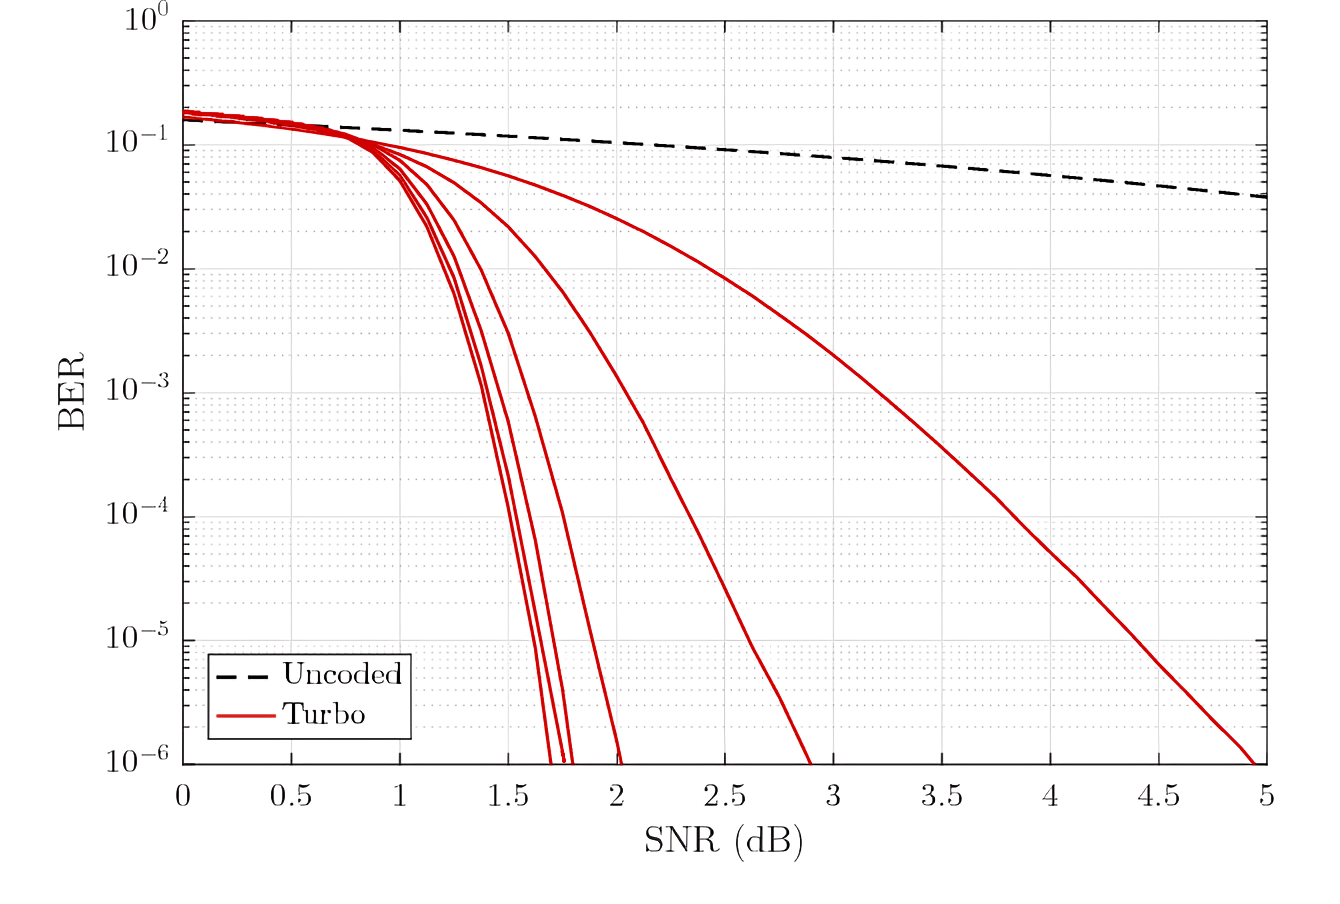
\includegraphics[width=0.5\textwidth]{imgs/turbo_code_ber.png}
\end{center}

In figura viene mostrata la convergenza con $K=2048$, $R=1/2$ e un numero di iterazioni, da sinistra a destra, pari rispettivamente a $32, 16, 8, 4, 2, 1$.


\section*{Space diversity}

In generale sia la frequency che time diversity richiedono parecchie risorse, per questo un altro tipo di diversity è spesso sfruttata, semplicemente utilizzando più antenne. Si possono sfruttare due tipologie di gain differenti:
\begin{itemize}
    \item \textbf{Array gain}: si tratta del guadagno di potenza ottenuto utilizzando più antenne rispetto all'utilizzo della singola antenna. Il guadagno è tanto più alto quanto è alta la correlazione spaziale del canale. Si sfruttano tipicamente antenne direzionali.
    \item \textbf{Diversity gain}: si tratta del guadagno ottenuto combinando i segnali ricevuti dalle varie antenne, considerati incorrelati. Tale guadagno è massimo quando i segnali sono completamente decorrelati. 
\end{itemize} 

Per assumere incorrelazione tra le varie antenne la loro distanza deve essere almeno la metà della lunghezza d'onda:
\[
    d_c = \frac{\lambda}{2} \quad \text{coherence distance}
\]  

La \textbf{coherence distance} deriva dalle proprietà di time varying del canale, tuttavia come si può osservare non ha dipendenze né dal tempo, né dalla velocità.

Le carrier frequencies attualmente utilizzate permettono di utilizzare anche antenne nel solito sistema sfruttando al massimo la space diversity. Bisogna comunque tenere in considerazione che ogni antenna ha bisogno della propria RF chain, quindi lo spazio occupato è maggiore rispetto alla grandezza dell'antenna.


\paragraph*{Canale MIMO (Multiple Input Multiple Output)}


Nei classici sistemi con un antenna in trasmissione ed un'antenna in ricezione, il canale, se narrow-band può essere descritto da uno scalare complesso.
Nel caso di sistemi con più antenne in trasmissione e ricezione tra ogni coppia di antenne vi è un canale differente, quindi l'intero sistema, per quanto riguarda il canale, può essere descritto tramite una mtrice complessa.
\[ 
    \mathbf{H} = 
    \begin{bmatrix}
        h_{11} & h_{12} & \ldots & h_{1M} \\
        h_{21} & h_{22} & \ldots & h_{2M} \\
        \vdots & \vdots & \ddots & \vdots \\
        h_{N1} & h_{N2} & \ldots & h_{NM} \\
    \end{bmatrix}
    , \quad
    \begin{array}{ll}
            \mathbf{H} \in \mathbb{C}^{N \times M} \\
            \mathbf{y} = \mathbf{Hx} 
    \end{array}
\]

Dove $\mathbf{x}$ è il segnale trasmesso, $\mathbf{y}$ è il segnale ricevuto e $\mathbf{H}$ è la matrice del canale. In questo caso, $M$ rappresenta il numero di antenne in trasmissione mentre $N$ il numero di antenne in ricezione.
\paragraph*{Canale SIMO (Single Input Multiple Output)}
\begin{center}
    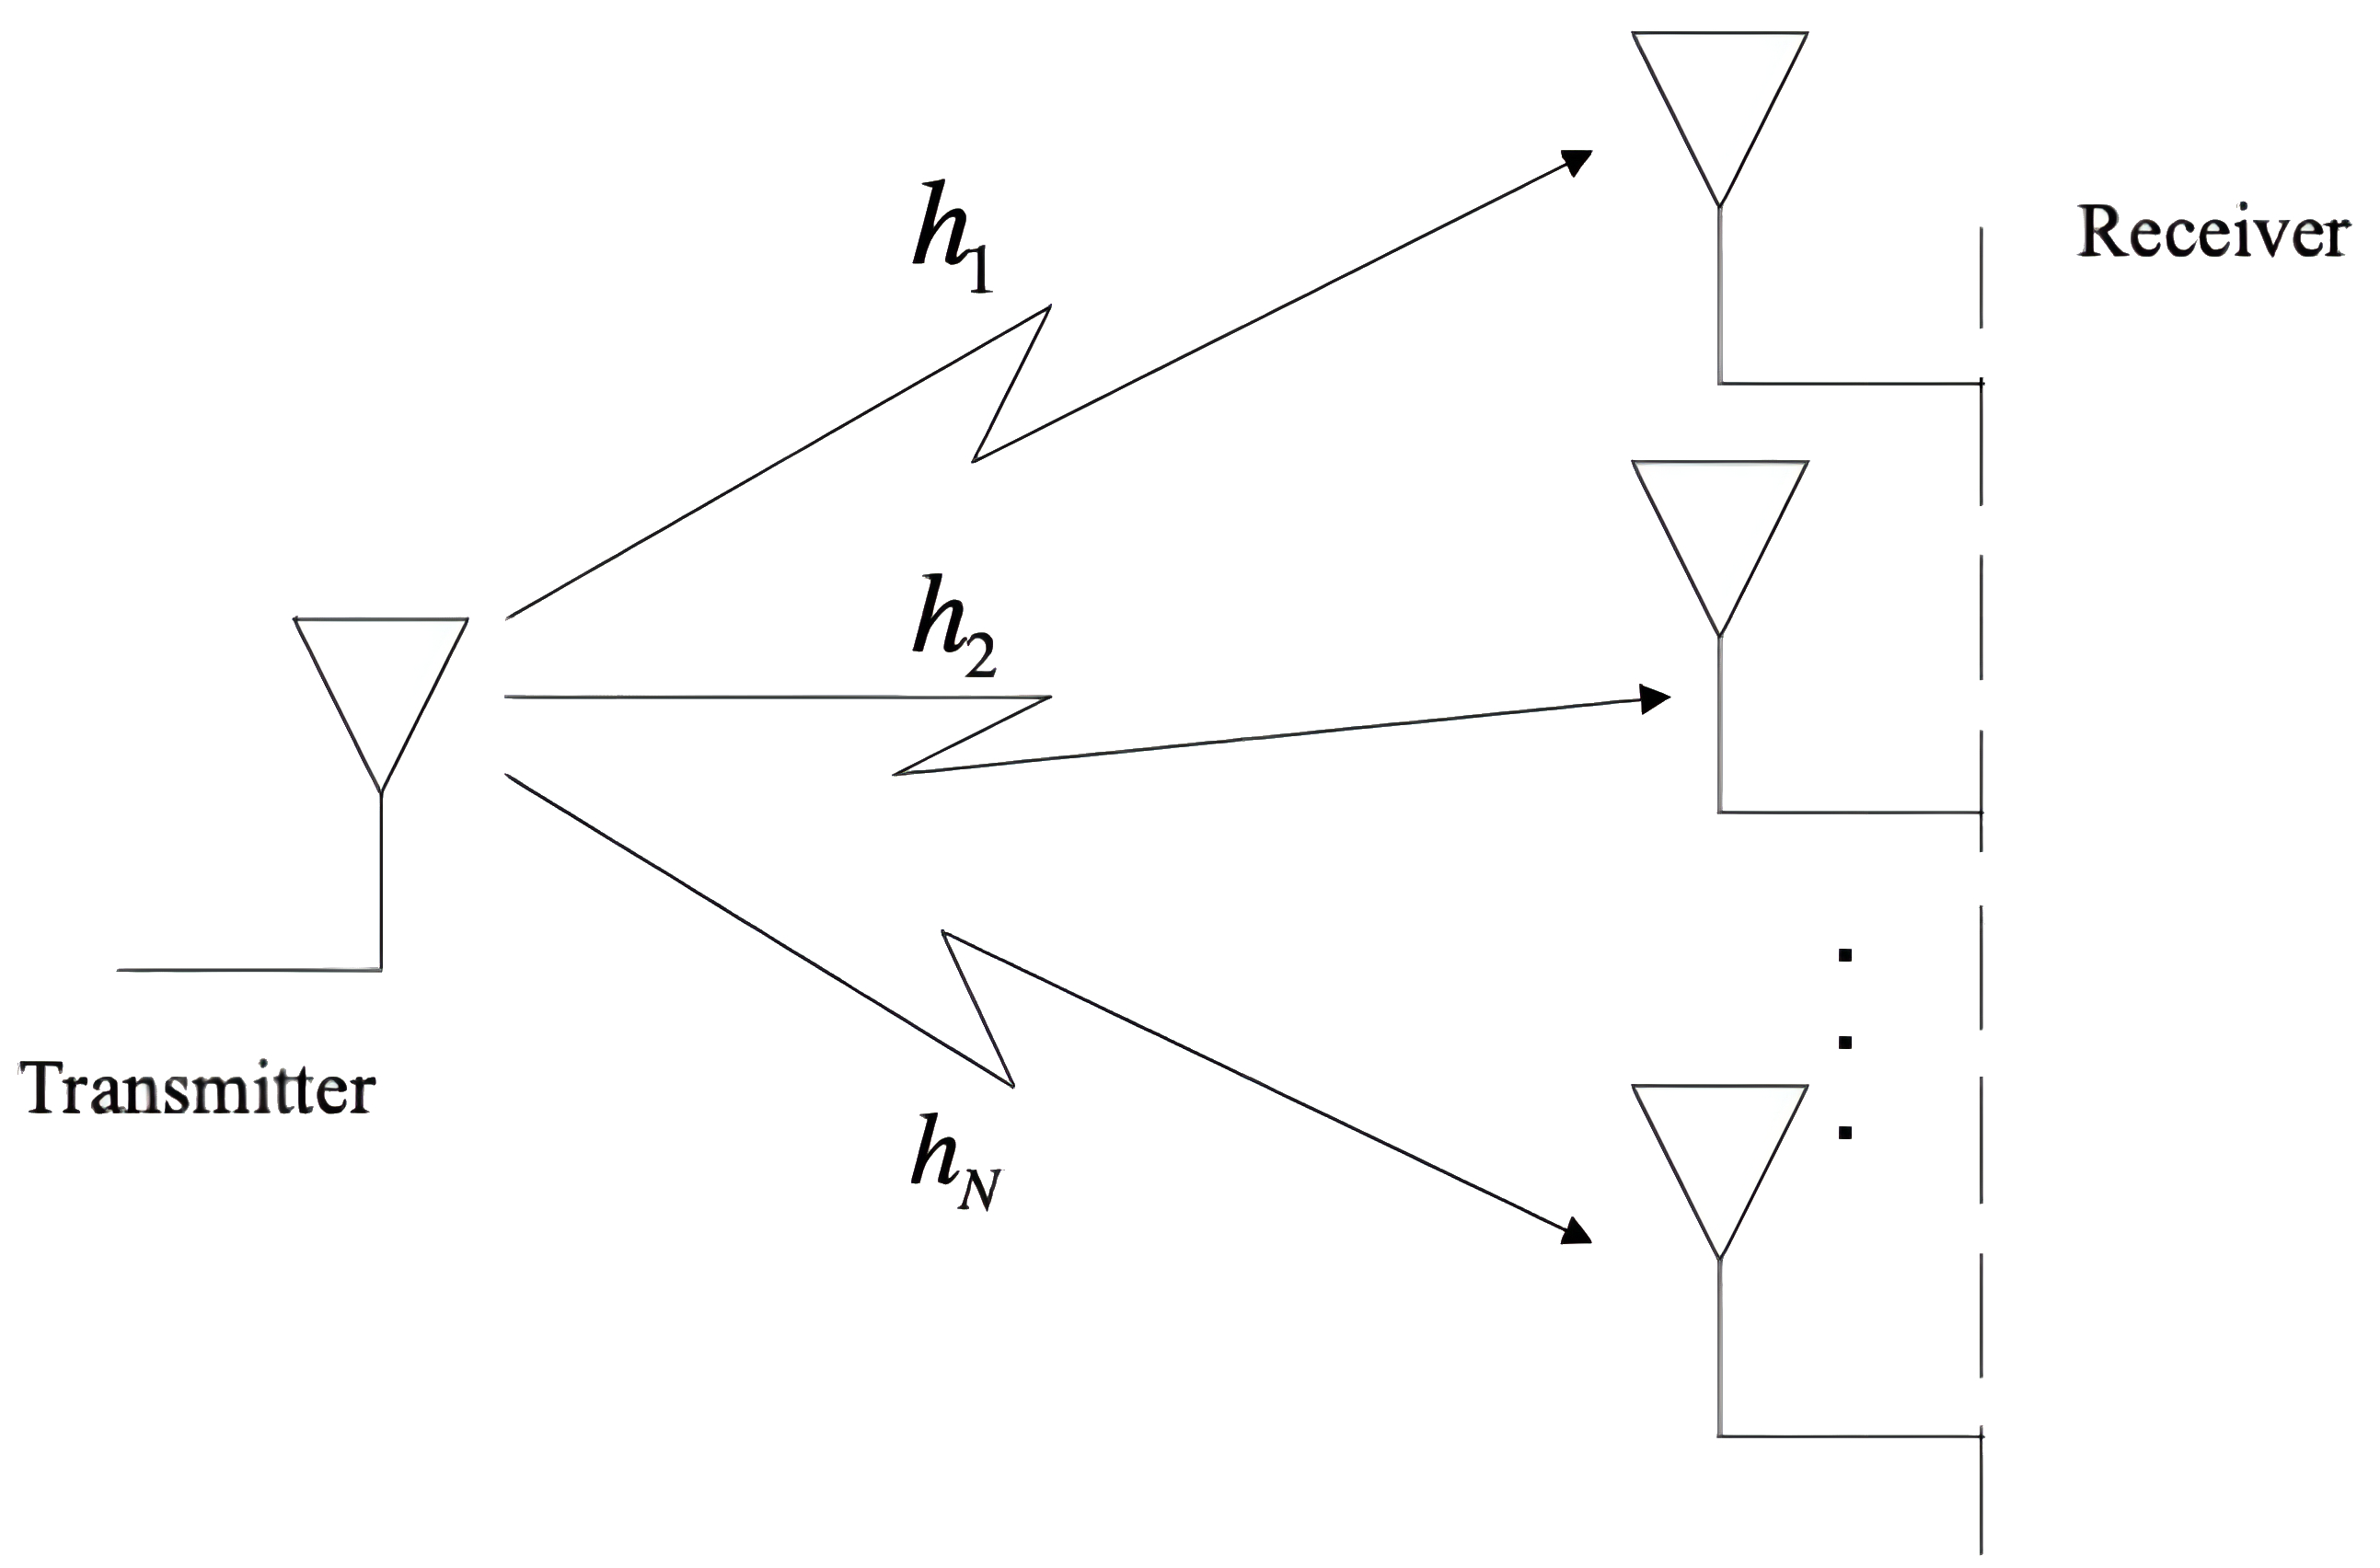
\includegraphics[width=0.4\textwidth]{imgs/simo.jpg}
\end{center}
Nel caso di unica antenna in trasmissione si parla di canale SIMO ed in tal caso $\mathbf{H} \in \mathbb{C}^{N \times 1}$
\[
    x_i[m] = h_i c_m + n_i[m] \quad i = 1, \ldots, N
\]
Questo rappresenta il segnale ricevuto sull'$i$-esima antenna.
È ragionevole assumere $h_i \in \mathbb{R}$ , dato che si può sempre moltiplicare $x_i[m]$ per $ e^{j\arg(h_i)} $ senza cambiare le statistiche del segnale.
Ogni segnale ha il proprio rumore e distorsione da parte del canale.

L'idea più semplice per sfruttare la diversity è scegliere di volta in volta il segnale con attenuzione minore, stimando il canale.
Tuttavia esistono tecniche in grado di utilizzare le informazioni provenienti da tutti i segnali ricevuti.
% TODO: i w_i sono reali o complessi 
\[
    z[m] = \sum_{i=1}^{N} w_i x_i[m] = \sum_{i=1}^{N} w_i h_i c_m + \sum_{i=1}^{N} w_i n_i[m]
\]
dove $w_i$ sono i pesi assegnati alle varie antenne.


% TODO: ma anche qui si moltiplica per l'opposto della fase?
\[
    P = \mathbb{E} \left[ \left| \sum_{i=1}^{N} w_i h_i c_m  \right|^2 \right] = \mathbb{E} \left[  |c_m|^2  \right] \left| \sum_{i=1}^{N} w_i h_i \right|^2 =  A \left| \sum_{i=1}^{N} w_i h_i \right|^2
\]

\[
    \begin{array}{ll}
            P_N = \mathbb{E} \left[ \left| \sum_{i=1}^{N} w_i n_i[m]  \right|^2 \right] \\
            = \mathbb{E} \left[ \left( \sum_{i=1}^{N} w_i n_i[m] \right)  \left( \sum_{i=1}^{N} w_i n_i[m] \right)^*  \right] \\
            = \mathbb{E} \left[  \sum_{i=1}^{N} \sum_{j=1}^{N} w_i w_j^* n_i[m] n_j[m]^*  \right] \\
            = \sum_{i=1}^{N} \sum_{j=1}^{N} w_i w_j^* \mathbb{E} \left[ n_i[m] n_j[m]^* \right] \\
            = \sum_{i=1}^{N} \sum_{j=1}^{N} w_i w_j^* \sigma^2 \delta_{ij} \\
            = \sum_{i=1}^{N} w_i w_i^* \sigma^2 \\
            = \sum_{i=1}^{N} |w_i|^2 \sigma^2 \\
            = \sigma^2 \sum_{i=1}^{N} |w_i|^2 
    \end{array}
\]

% TODO: come si rimuovono i complessi?
L'obiettivo è massimizzare il SNR, che si può quindi scrivere come:
\[
    \text{SNR} = \frac{P}{P_N} = \frac{A}{\sigma^2} \frac{\left|\sum_{i=1}^{N} w_i h_i \right|^2}{\sum_{i=1}^{N} \left| w_i \right|^2} \leq \frac{A}{\sigma^2} \frac{\sum_{i=1}^{N} |w_i|^2 \sum_{i=1}^{N} \left| h_i \right|^2}{\sum_{i=1}^{N} |w_i|^2} = \frac{A}{\sigma^2} \sum_{i=1}^{N} |h_i|^2
\]

dove la disuguaglianza è dovuta alla disuguaglianza di Schwarz. Imponendo la condizione $w_i = h_i^*$ si ottiene il massimo SNR possibile e quindi vale l'uguaglianza:
\[ 
    \text{SNR} = \frac{A}{\sigma^2} \frac{\left(\sum_{i=1}^{N} \left| h_i \right|^2 \right)^2}{\sum_{i=1}^{N} \left| h_i^2 \right|} = \frac{A}{\sigma^2} \sum_{i=1}^{N} |h_i|^2
\]


% TODO: h è complesso? Nel caso vi vuole il modulo?
Se si ha un unico canale l'espressione del SNR si riduce al semplice rapporto $\frac{A}{\sigma^2}h$, ovvero la forma valida per un semplice fading channel.
\paragraph*{MISO (Multiple Input Single Output)}
\begin{center}
    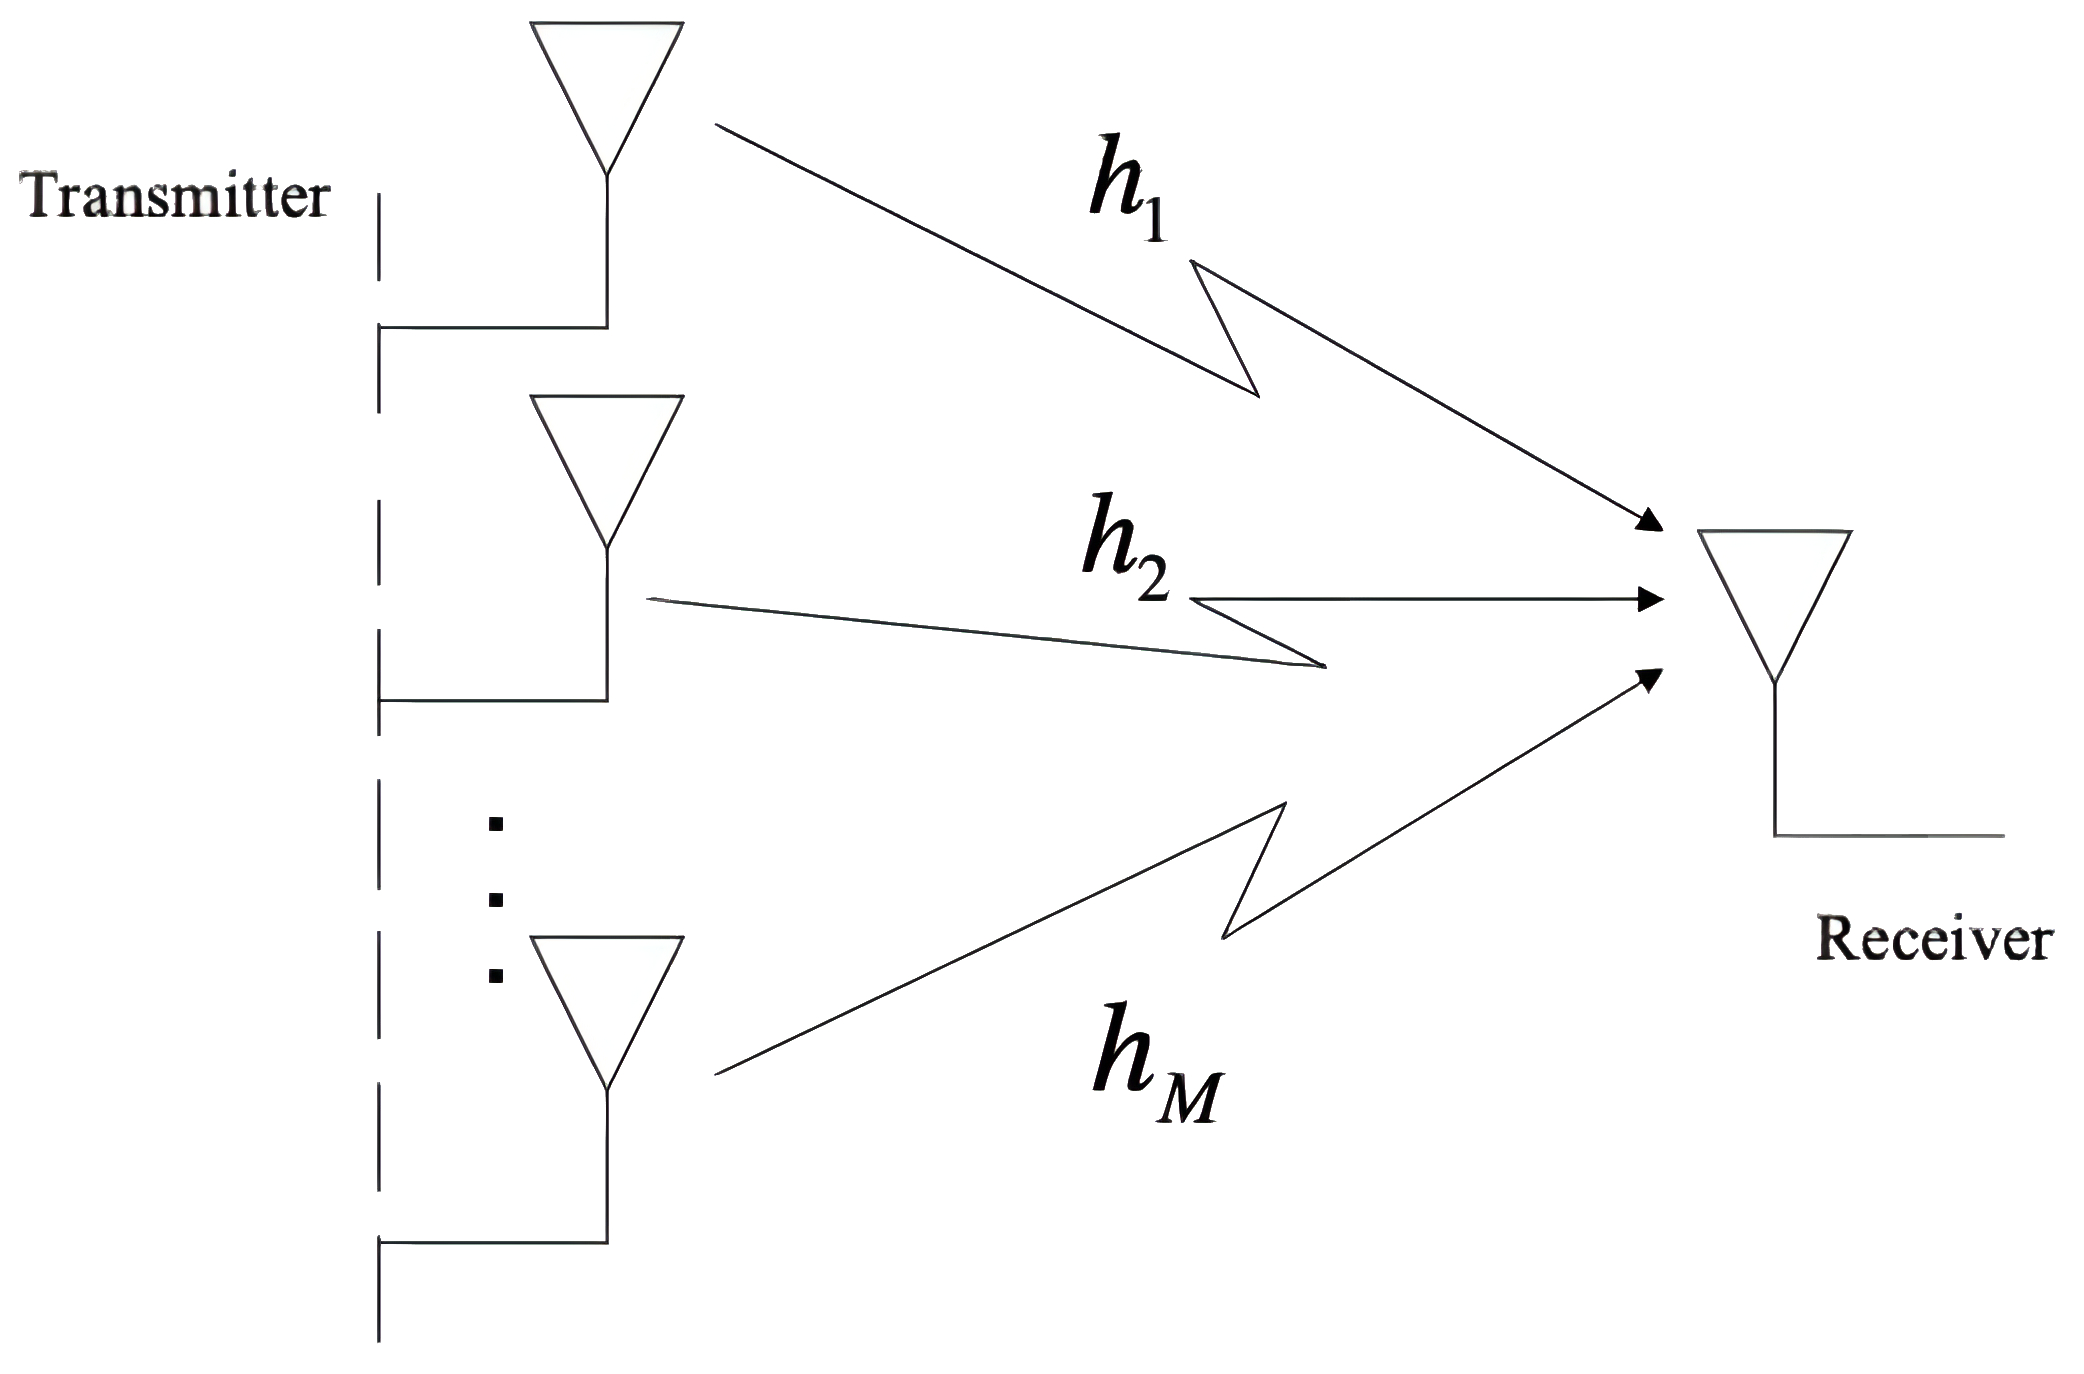
\includegraphics[width=0.4\textwidth]{imgs/miso.jpg}
\end{center}
Per quanto riguarda la configurazione con più antenne in trasmissione e singola antenna in ricezione, sistema MISO, si ottiene la stessa espressione con alcuni accorgimenti lato trasmettitore
\[
    x[m] = \sum_{i=1}^{N} h_i y_i[m] + n[m] \quad \text{segnale ricevuto tramite l'unica antenna disponibile}
\]


La differenza sostanziale con il caso SIMO è che i vari segnali sono combinati ``naturalmente" durante la trasmissione e ricevuti quindi già aggregati. 
La scelta dei coefficienti non può essere effettuata lato ricevitore, ma deve essere il trasmettitore a scegliere stimando il canale, lato ricevitore la stima è ovviamente più complessa rispetto a quella che effettuerebbe il ricevitore per proprio conto.
L'operazione effettuata dal trasmettitore è detta \textbf{spatial precoding} ed il simbolo è denominato \textbf{spatial pre-coded symbol}.
\[
    y_i[m] = b_i c_m \quad \text{simbolo trasmesso sulla $i$-esima antenna}
\]
L'energia spesa dipende anche dal coefficiente $b_i$, l'obiettivo è comunque utilizzare la solita energia usata nel caso di singola antenna.

Il rapporto SNR è massimizzato scegliendo $b_i = \frac{h_i^*}{ \| \mathbf{h} \| }$

\[
    x[m] = \sum_{i=1}^{N} h_i y_i[m]  = \sum_{i=1}^{N} h_i b_i c_m + n[m] = \sum_{i=1}^{N} \frac{h_i h_i^*}{\| \mathbf{h} \|} c_m + n[m] = \| \mathbf{h} \| c_m + n[m]
\]
\[
    P = \|\mathbf{h} \|^2 \ \mathbb{E} \left[\left| c_m \right|^2 \right] = \|\mathbf{h} \|^2  A
\]
\[
    P_N = \sigma^2  
\]
\[
    \text{SNR} = \frac{P}{P_N} = \sum_{i=1}^{N} |h_i|^2 \frac{A}{\sigma^2}    
\]
% TODO: ma h_i è un parametro o una variabile aleatoria?
La differenza tra il caso con singola antenna (sia lato trasmettitore che ricevitore) e il caso con più antenne (MISO/SIMO) è dato dal fattore $\| \mathbf{h} \| = \sum_{i=1}^{N} |h_i|^2$.
Considerando i guadagni del canale come variabili aleatore con distribuzione di Rayleigh è possibile calcolare la distribuzione della somma come convoluzione delle PDF.
\[
    f_{\| \mathbf{h} \|^2} (x) = \frac{1}{D-1} x^{D-1} e^{-x}
\]
Il risultato dipende dal nnumero di antenne, tuttavia in generale si ottiene un \textbf{array gain}, ovvero uno spostamente del valor medio dei gain verso destra (più potenza).
Inoltre il \textbf{diversity gain} si manifesta riducendo notevolmente la probabilità di ottenere guadagni molto bassi.
Ciò è visibile confrontando gli integrali delle due PDF.

\paragraph*{MIMO (Multiple Input Multiple Output)}

Il caso generale MIMO, ovvero con più antenne sia in trasmissione che ricezione, sfrutta una tecnica denominata \textbf{spatial multiplexing} ed è basata sulla decomposizione ai valori singolari (SVD) della matrice $\mathbf{H}$ che descrive il canale.

\paragraph*{SVD (Singular Value Decomposition)}

Data una matrice $\mathbf{A} \in \mathbb{C}^{m \times n}$, con  $p = \text{rank} (\mathbf{A})$, la SVD permette di scrivere la matrice come prodotto di tre matrici:
\[
    \mathbf{A} = \mathbf{U} \mathbf{\Sigma} \mathbf{V}^H
\]
con $\mathbf{U} \in \mathbb{C}^{m \times p}$, $\mathbf{\Sigma} \in \mathbb{C}^{p \times p}$ e $\mathbf{V} \in \mathbb{C}^{n \times p}$,
dove $\mathbf{U}$ e $\mathbf{V}$ sono matrici unitarie, mentre $\mathbf{\Sigma} = diag(\sigma_1, \ldots, \sigma_p)$ è una matrice diagonale con $\sigma_1 \geq \sigma_2 \geq \ldots \geq \sigma_p$. In un sistema MIMO, se il canale è sufficientemente multipath, la matrice $\mathbf{H}$ ha rango pieno, dunque:
\[
    p = \text{rank}(H) = \min(N_R, N_T)
\]

La tecnica di \textbf{spatial multiplexing} consiste nell'effettuare sia un pre-coding lato trasmettitore, sia un combining lato ricevitore, dunque utilizzando due pesi differenti. In questo modo è possibile creare un certo numero di canali ortogonali indipendenti, detti \textbf{spatial channels}.
\[
    \begin{array}{ll}
        \mathbf{H} = \mathbf{U} \mathbf{\Sigma} \mathbf{V}^H \quad \text{decomposizione SVD matrice del canale MIMO} \\
        \mathbf{B} = \mathbf{V} \quad \text{matrice pre-coder (Tx)} \\
        \mathbf{W} = \mathbf{U} \quad \text{matrice combiner (Rx)}
    \end{array}
\]
\begin{center}
    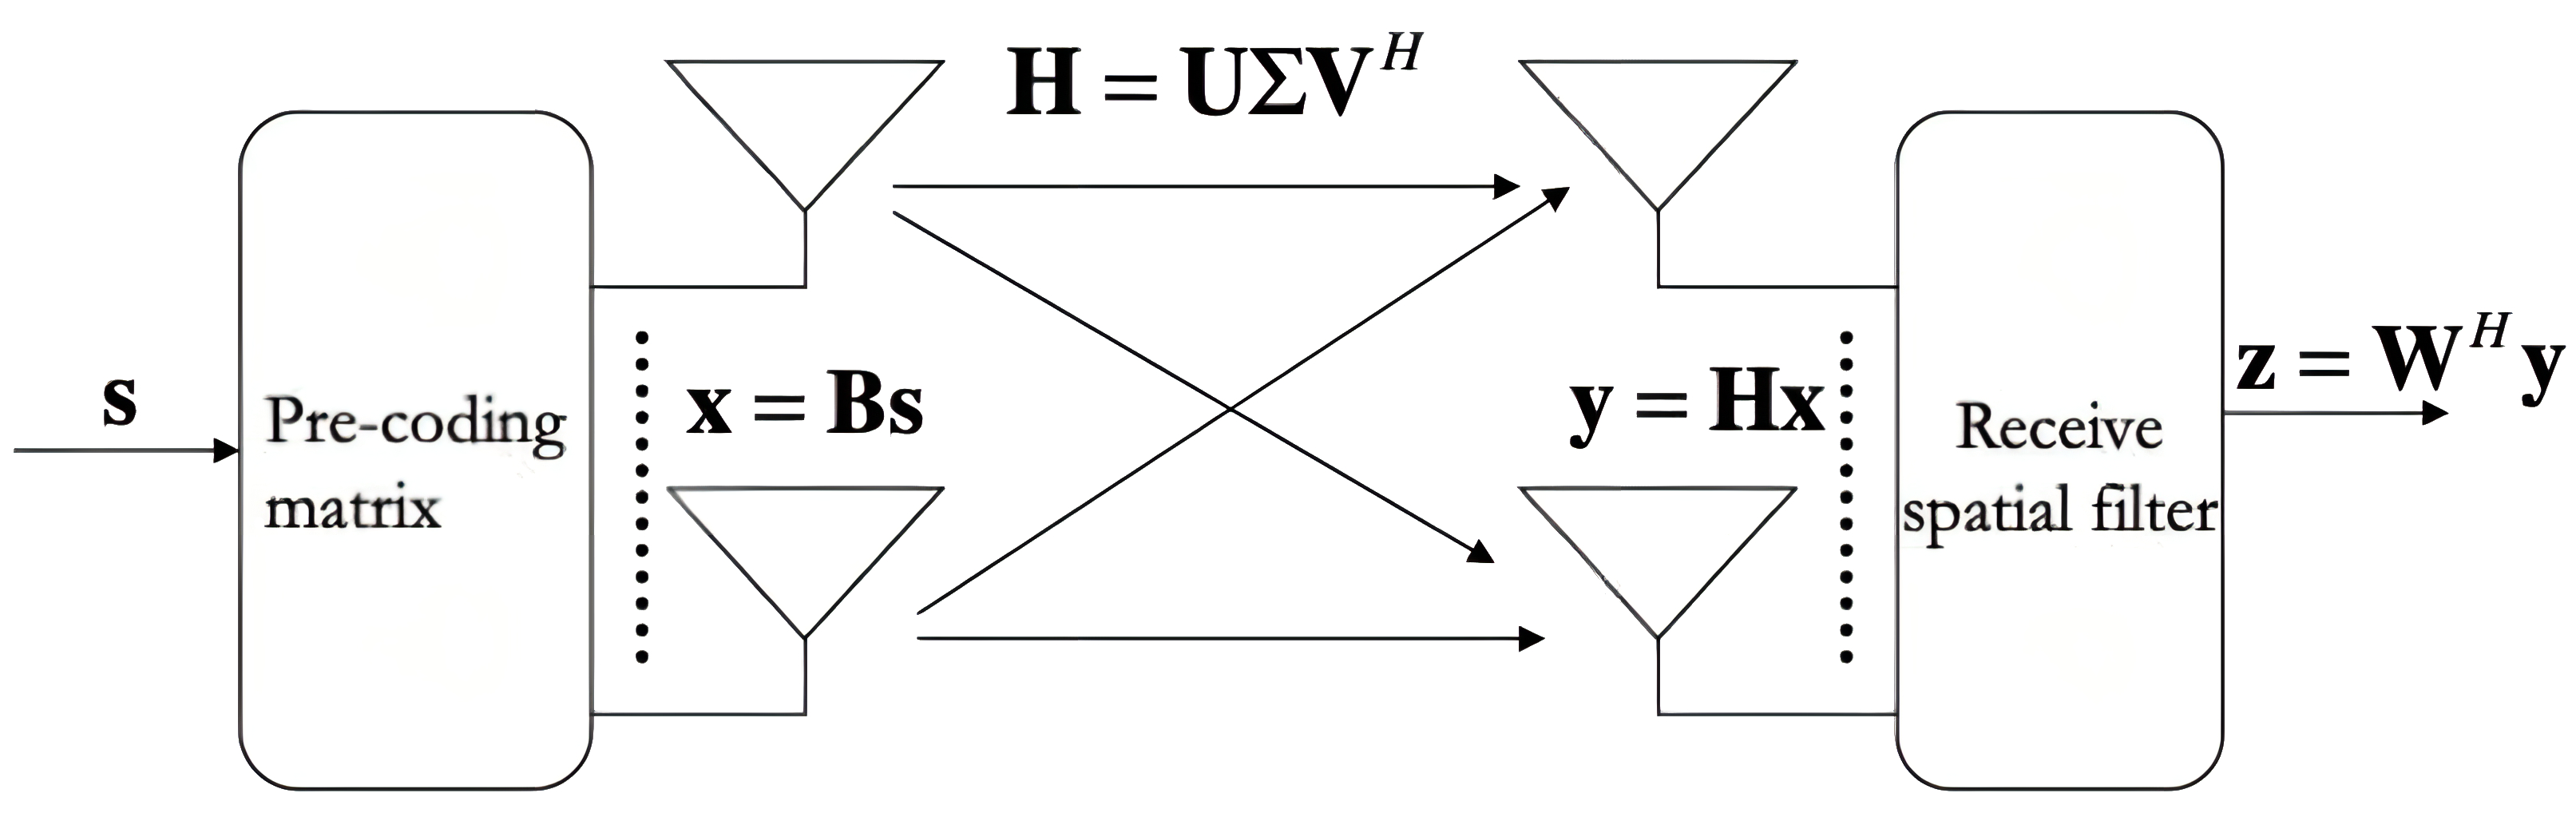
\includegraphics[width=0.8\textwidth]{imgs/mimo.jpg}
\end{center}

Scegliendo in questo modo le matrici si ottiene:
\[
    \begin{array}{ll}
        \mathbf{z} = \mathbf{W}^H \mathbf{y}  \\
        = \mathbf{W}^H \left( \mathbf{H} \mathbf{x} + \mathbf{n}  \right) \\  
        = \mathbf{W}^H \left( \mathbf{H} \mathbf{B} \mathbf{s} + \mathbf{n} \right) \\
        = \mathbf{W}^H \mathbf{H} \mathbf{B} \mathbf{s} + \mathbf{W}^H \mathbf{n}  \\
        = \mathbf{U}^H \mathbf{H} \mathbf{V} \mathbf{s} + \mathbf{W}^H \mathbf{n} \\
        = \mathbf{\Sigma} \mathbf{s} + \mathbf{W}^H \mathbf{n}
    \end{array}
\]
Sebbene ogni antenna riceva dei segnali sovrapposti, scegliendo le matrici in questa maniera è possibile ottenere dei canali ortogonali che non interferiscono tra loro dato che la matrice $\mathbf{\Sigma}$ è diagonale.

Considerando un sistema $2 \times 2$ per esempio si ottiene:
\[
    \begin{cases*}
        y_1 = h_{11} x_1 + h_{12} x_2 + n_1 \\
        y_2 = h_{21} x_1 + h_{22} x_2 + n_2
    \end{cases*}
    \quad
    \text{segnali sovrapposti su ogni antenna}
\]

L'utilizzo di un canale MIMO può incrementare la capacità del sistema, tuttavia è necessario tenere in considerazione anche i valori singolari, i quali potrebbero comportare un'attenuazione eccessiva.


\[
    \mathbf{z} = \begin{matrix}
        \begin{bmatrix}
            \sigma_1 s_1 + n_1' \\
            \sigma_2 s_2 + n_2'
        \end{bmatrix}
    \end{matrix}
    \quad 
    \text{segnale ottenuto dopo combining lato ricevitore, non c'è alcuna sovrapposizione}
\]


% TODO: aggiungere considerazioni sull'aumento della capacità del sistema


\section*{Frequency diversity}

La formula di Shannon fornisce il massimo rate sostenibile su un dato canale di trasmissione:
\[
    C = B \log_2 \left( 1 + \text{SNR} \right), \quad \text{SNR} = \frac{\left| H \right|^2 P}{\sigma^2}
\]
Dove $H$ è il guadagno del canale.
In sistemi reali ci si può solo avvicinare al limite teorico e vi è una forte dipendenza, per quanto riguarda l'efficienza spettrale, del coding rate e modulation order, data dalla dimensione della costellazione di simboli per cui esiste un trade-off tra capacità di trasmissione ed energia richiesta.
In particolare $\log_2 \left( 1 + \text{SNR} \right)$ è l'efficienza spettrale.
Il rate di trasmissione reale può essere approssimato:
\[
    R_b = \log_2 M \  R \frac{1}{T}  \approx m R B
\]

Dove è $M$ è il numeri di simboli nella costenllazione, $R$ è il coding rate \footnote{con $R_s$ indichiamo il symbol rate, ovvero $\frac{1}{T}$, mentre con $R$ il symbol rate} e $T$ è il symbol time, si fa l'approssimazione che $\frac{1}{T} \approx B$. 


Per rispettare il limite di capacità si deve avere:
\[
    m R B < C \quad \Rightarrow \quad m R < \log_2 (1 + \text{SNR})
\]
Misurando il SNR è possibile adattare i valori di $m$ ed $R$, ad esempio in base alla posizone in una cella.
I valori di $m$ ed $R$ che si possono utilizzare appartengono ad un insieme finito, non è possibile scegliere arbitrariamente.

\begin{table}[H]
    \resizebox{\textwidth}{!}{
        \centering
        \begin{tabular}{|c|l|c|c|c|}
        \hline
        \textbf{Radio Bearer Index} & \textbf{Name} & \textbf{Modulation} & \textbf{Channel Coding Rate} & \textbf{Bearer Efficiency} ($\log_2(1+\text{SNR})$, bits/symbol) \\ \hline
            1  & QPSK 1/12 & QPSK & 0.0761719 & 0.1523 \\ \hline
            2  & QPSK 1/9  & QPSK & 0.117188  & 0.2344 \\ \hline
            3  & QPSK 1/6  & QPSK & 0.188477  & 0.377  \\ \hline
            4  & QPSK 1/3  & QPSK & 0.300781  & 0.6016 \\ \hline
            5  & QPSK 1/2  & QPSK & 0.438477  & 0.877  \\ \hline
            6  & QPSK 3/5  & QPSK & 0.587891  & 1.1758 \\ \hline
            7  & 16QAM 1/3 & 16QAM & 0.369141  & 1.4766 \\ \hline
            8  & 16QAM 1/2 & 16QAM & 0.478516  & 1.9141 \\ \hline
            9  & 16QAM 3/5 & 16QAM & 0.601563  & 2.4063 \\ \hline
            10 & 64QAM 1/2 & 64QAM & 0.455078  & 2.7305 \\ \hline
            11 & 64QAM 1/2 & 64QAM & 0.553711  & 3.3223 \\ \hline
            12 & 64QAM 3/5 & 64QAM & 0.650391  & 3.9023 \\ \hline
            13 & 64QAM 3/4 & 64QAM & 0.753906  & 4.5234 \\ \hline
            14 & 64QAM 5/6 & 64QAM & 0.852539  & 5.1152 \\ \hline
            15 & 64QAM 11/12 & 64QAM & 0.925781  & 5.5547 \\ \hline
        \end{tabular}
    }
\end{table}

Come si evince dala tabella, in pratica c'è un mapping diretto tra SNR misurato (channel quality indicator, CQI) e lo specifico ordine di modulazione e coding rate di una trasmissione.
La qualità del canale in termini di SNR può essere espressa tramite \textbf{radio beared index} ($\in [1, 15]$).
Utilizzando la modulazione OFDM l'idea sarebbe adattare $m$ ed $R$ per ogni canale, distribuendo la potenza nel modo più efficace possibile per massimizzare il rate di trasmmissione. Questo problema è inidcato con il termine di \textbf{water-filling}, la potenza a disposizione è invece detta \textbf{power budget}. Nella pratica si tratta di un problema di ottimizzazione per il quale sono definiti alcuni vincoli da rispettare:

% TODO: p non lo metterei, perché non è chiaro cosa rappresenti
\[
    \begin{cases}
       \underset{\mathbf{p}}{\text{max}} \sum_{n=1}^{N} \log_2(1 + \frac{P_n}{\sigma_n^2}), \quad P_n \geq 0 \quad n = 1, \ldots, N \\
       \sum_{n=1}^{N} P_n = P_0 \quad \text{(power budget)} \\
        P_n \geq 0 \quad n = 1, \ldots, N
    \end{cases}    
\]

Dove $\sigma_n^2 = \frac{\sigma^2}{\left| \mathbf{H}_{n, n} \right| ^2}$. Il termine $B$ non appare nell'espressione in quanto costante per ogni canale, massimizzare il rate o l'efficienza spettrale genera lo stesso risultato.

La lagrangiana del problema è:
\[
    \mathcal{L}(P_1, \hdots, P_N, \lambda ) = \sum_{n=1}^{N} \log_2(1 + \frac{P_n}{\sigma_n^2}) - \lambda \left( \sum_{n=1}^{N} P_n - P_0 \right)
\]
La derivata rispetto a $P_n$ posta a 0 per la condizione di stazionarietà è:
\[
    \frac{\partial \mathcal{L}}{\partial P_n} = \frac{1}{\ln(2)} \frac{1}{1 + \frac{P_n}{\sigma_n^2}} \frac{1}{\sigma_n^2} - \lambda = 0, \quad n = 1, \ldots, N
\]
overro il gradiente:
\[
    \nabla_{P_1, \hdots, P_N} \mathcal{L} = \begin{bmatrix}
        \frac{1}{\ln(2)} \frac{1}{1 + \frac{P_1}{\sigma_1^2}} \frac{1}{\sigma_1^2} - \lambda \\
        \frac{1}{\ln(2)} \frac{1}{1 + \frac{P_2}{\sigma_2^2}} \frac{1}{\sigma_2^2} - \lambda \\
        \vdots \\
        \frac{1}{\ln(2)} \frac{1}{1 + \frac{P_N}{\sigma_N^2}} \frac{1}{\sigma_N^2} - \lambda \\
\end{bmatrix} = \mathbf{0}
\]

La soluzione del problema è:
\[
    \hat{P}_n = \frac{1}{\lambda \ln(2)} - \sigma_n^2, \quad n = 1, \ldots, N
\]
considerando il vincolo che $P_n \geq 0$ e ponendo $\mu = \frac{1}{\lambda \ln(2)}$ si ottiene:
\[
    \hat{P}_n = \text{max} \{ 0, \mu - \sigma_n^2    \} = (\mu - \sigma_n^2)^+, \quad n = 1, \ldots, N
\]

Per ottenere dei valori è necessario calcolare $\mu$, scelto in modo da rispettare il vincolo sulla potenza a disposizione.
\[
    \sum_{n=1}^{N} (\mu - \sigma_n^2)^+ = P_0
\]
\[
    \begin{cases}
        f(\mu) = \sum_{n=1}^{N} (\mu - \sigma_n^2)^+ - P_0 \\
        f: \mathbb{R}^n \rightarrow \mathbb{R}
    \end{cases}
\]
La risoluzione dell'equazione garantisce il valore $\mu$ tale per cui i vincoli sono rispettati, è quindi necessario trovare lo zero di una funzione in $\mu$, ad esempio con il metodo della bisettrice.
Il metodo dei bisezione può essere applicato dato che la funzione risulta continua e monotona su% TODOl dominio.
Il termine water-filling deriva dal fatto che osservando il grafico della distribuzione della potenza, si ha l'impressione che la potenza si distribuisca come l'acqua all'interno di un contenitore con superiore irregolare, fino ad un livello pari a $\mu$.
La distribuzione è ottima e rappresenta la miglior situazione per sfruttare la frequency diversity del canale.
In sostanza la distribuzione favorisce i canali con miglior qualità, scartando completamente quelli la cui capacità è troppo bassa.



% TODO: aggiungere qualcosa sul waterfilling


% TODO: la fft size è 2048 come il numero di subcarriers?

La banda di un singolo subcarrier è calcolata come:
\[
    \Delta f = \frac{f_s}{N} = \frac{30.72 \text{ MHz}}{2048} = 15 \text{ kHz}
\]
La banda di un resource block (RB), cioè la minima unità allocabile, è calcolata come:
\[
    B_{RB} = 12 \times 15 \text{ kHz} = 180 \text{ kHz}
\]
La raw bandwidth è calcolata come:
\[
B_{raw} = 1200 \times 15 \text{ kHz} = 18 \text{ MHz}
\]
La disponibilità di banda è calcolata togliendo dalla banda grezza la banda usata per informazioni di sincronizzazione e controllo:
\[
B_{av} = B_{raw} - 4 \text{ MHz} = 14 \text{ MHz}
\]
Il rate massimo per un canale SISO è:
\[
    R_{1 \times 1} = 0.9258 \times 8 \times 14 \text{ MHz} \approx 100 \text{ Mb/s}
\]
Con il carrier aggregation: quando gli operatori comprano lo spettro di trasmissione, compratno chunks dello spettro che sono più larghi di 20 MHz, e possono essere aggreagati per un singolo utente
Con un canale MIMO $4 \times 4$ si ha un massimo data rate di:
\[
    R_{4 \times 4} = 4 \times 0.9258 \times 8 \times 14 \text{ MHz} \approx 400 \text{ Mb/s}
\]


I terminali più avanzati possono aggregare più bande da 20 MHz ciascuna, per esempio 3 con $4 \times 4$ MIMO e 2 con $2 \times 2$ MIMO, ottenendo un rate di:
\[
    R_{\text{aggregated}} = 3 \times 400 \text{ Mb/s} + 2 \times 200 \text{ Mb/s} = 1.6 \text{ Gb/s}
\]


\section*{Transmissions over Fading Channels}

\begin{itemize}
    \item Signal fading is the main problem in wireless communications.
    \item OFDM is a technique designed to combat the destructive effects of multipath fading.
    \item Slow flat Rayleigh fading is still a big problem.
    \item One of the most effective resources against the effects of channel fading is \textbf{diversity}.
\end{itemize}

\section*{Diversity in Wireless Communications}

\begin{itemize}
    \item \textbf{Diversity} refers to the possibility of improving the reliability of a message by transmitting it over two or more communication channels with different characteristics.
    \item Diversity is a common technique for combatting fading and co-channel interference and avoiding error bursts.
\end{itemize}


\section*{Diversity in Wireless Communication Systems}

\subsection*{Time Diversity:}
Time diversity relates to the \textit{coherence time} of the channel and includes techniques such as transmission over multiple time slots by channel coding plus interleaving. It is particularly effective over very slow fading channels.

\subsection*{Frequency Diversity:}
Frequency diversity relates to the \textit{coherence bandwidth} of the channel. It involves transmission over multiple frequency bands and offers advantages over very flat fading channels.

\subsection*{Spatial Diversity:}
Spatial diversity is associated with the \textit{coherence distance} and involves the transmission and reception employing multiple antennas.

\section*{Time Diversity: Interleaving and Coding}
\begin{itemize}
    \item Initially proposed by Claude Shannon in 1948, channel coding introduces redundancy to detect errors at the receiver and improve the bit error probability.
    \item Redundancy is quantified by the code rate $R = \frac{k}{n}$, where $k$ is the number of input bits, and $n$ is the number of output bits from the encoder.
    \item While initially studied for AWGN channels, channel codes are applicable to fading channels to enhance reliability.
\end{itemize}



\section*{Error Detection Coding}

A straightforward technique in error detection is the use of parity bits. Parity bits are additional bits at the end of a data word used for error detection. They provide a simple way to check the integrity of the data. 

\subsection*{Parity Check Code}
A parity check code is an error detection code where the code rate \( R \) is determined by the ratio of information bits to total bits, including the parity bit(s). 

For example, consider a parity check code with rate \( R = \frac{7}{8} \):
\begin{itemize}
    \item The word is composed of \( k = 7 \) bits.
    \item A single parity bit is added, making \( n = 8 \) bits in total.
    \item The generator matrix \( \mathbf{G} \) for such a code can be expressed as a \( 7 \times 8 \) matrix, where the additional column is used for the parity bit, ensuring that the word always contains an even number of '1's.
    \item The encoded vector \( \mathbf{d} \) is then given by \( \mathbf{d} = \mathbf{uG} \), where \( \mathbf{u} \) is the vector of information bits.
\end{itemize}

The encoded word is an 8-bit vector with the property that it contains an even number of '1's if the original 7-bit word contained an odd number of '1's, and vice versa.

At the decoder side:
\begin{itemize}
    \item The receiver computes the parity check by examining the number of '1's in the received 8-bit word.
    \item If the number of '1's is even, the word is considered error-free.
    \item If the number of '1's is odd, this indicates that an error has occurred, assuming only single-bit errors are possible.
\end{itemize}

Not all errors can be detected with this method, particularly if an even number of bits are in error, as this will not affect the parity check condition.


\section*{Data Retransmission and Channel Capacity}

\subsection*{Data Retransmission}
\begin{itemize}
    \item Automatic Repeat Request (ARQ) is a protocol for error control in data transmission where the receiver sends back an acknowledgment (ACK) for correctly received packets and a negative acknowledgment (NACK) for faulty ones.
    \item When a NACK is received, the transmitter resends the data packet. This method exploits the \textit{time diversity} of the channel by retransmitting the data after a time interval longer than the channel coherence time \( T_c \).
    \item Advanced receivers can combine multiple received messages to improve the chances of successful reception, known as \textit{diversity combining}.
\end{itemize}

\subsection*{Error Correction Coding and Channel Capacity}
\begin{itemize}
    \item Error correction coding is utilized to correct errors introduced by the channel during transmission.
    \item Shannon's theorem establishes that for a communication channel of bandwidth \( B \), the channel capacity \( C \) is the upper bound on the rate at which information can be reliably transmitted over the channel and is given by:
    \[ C = B \log_2 (1 + \text{SNR}) \text{ bits/s}, \]
    where SNR is the Signal-to-Noise Ratio.
    \item If the transmission rate \( R \) is less than the channel capacity \( C \), it is theoretically possible to design an error correction code that makes the probability of error as low as desired, but not zero.
    \item On the contrary, if \( R > C \), it is impossible to guarantee an arbitrarily low error probability.
\end{itemize}

\subsection*{Practical Example}
\begin{itemize}
    \item In a communication system with bandwidth \( B = 1.8 \) MHz and using 16-QAM modulation, if the symbol rate \( R_s = \frac{1}{T} \) is such that \( R_s \cdot B \log_2(1 + \text{SNR}) \) does not exceed \( 40 \) Mbits/s, the transmission is within the channel capacity and is thus feasible.
    \item Otherwise, if the product of symbol rate and channel capacity is exceeded, the transmission would exceed the channel's capability to convey information without errors, leading to an increased error rate.
\end{itemize}






\section*{Block Codes: Repetition Code and Decoding}

\subsection*{Repetition Code}
\begin{itemize}
    \item The simplest form of block codes is the repetition code.
    \item For \( k = 1 \) and \( n = 3 \), the \( 3 \)-repetition code is used, which can be considered as a \( (1,3) \) code.
    \item The generator matrix for the code is \( G = \begin{bmatrix} 1 & 1 & 1 \end{bmatrix} \).
    \item Encoding of a bit \( u \) is done as \( d = uG \), resulting in \( d \) being either \( [0 \, 0 \, 0] \) or \( [1 \, 1 \, 1] \) for \( u = 0 \) or \( u = 1 \), respectively.
\end{itemize}

\subsection*{Decoder Operation}
\begin{itemize}
    \item The decoder uses majority decision decoding.
    \item Given a received bit string \( \hat{d} \), the decoder computes \( u = \hat{d} G^T \) and makes a decision based on the majority of bits.
    \item The rate \( R \) of the repetition code is \( \frac{1}{3} \).
\end{itemize}

\subsection*{Hamming Distance and Error Detection}
\begin{itemize}
    \item The Hamming distance is utilized to measure the distance between two codewords.
    \item For error detection, \( \hat{d} \) is chosen such that the Hamming distance \( d(\hat{d},d) \) is minimized.
    \item The Hamming distance provides a measure of error correction capability and error detection.
\end{itemize}


\section*{Block Codes: Decoder}

\begin{itemize}
    \item \textbf{Error Events:} An error event in block codes occurs when noise causes the received vector \(\hat{x}\) to be closer to a codeword that is different from the transmitted one.
    \item \textbf{Robustness of Codes:} Codes that have a larger Hamming distance between words are more robust against noise and fading compared to codes with a smaller Hamming distance.
    \item \textbf{Hamming Distance:} The Hamming distance is a metric that increases with the length of the code, specifically the parameters \(k\) (number of information bits) and \(n\) (length of the codeword). Unfortunately, the complexity of the receiver that must decode these codes also grows with \(k\).
\end{itemize}

\section*{Implications on Decoder Complexity}

The robustness of error-correcting codes and the ability of a decoder to correct errors without requiring retransmission are essential for efficient communication systems. However, this error correction capability comes at the cost of increased receiver complexity. This complexity is influenced by factors such as the length of the codeword \(n\) and the number of information bits \(k\). As these parameters increase, the computational effort required to decode the received messages also increases, which can impact the processing speed and energy consumption of communication devices.


\section*{Convolutional Codes: Encoder}

\begin{itemize}
    \item The encoder of a convolutional code, denoted as \((n, k, L)\), operates as \(n\) parallel linear filters over the Galois field GF(2).
    \item The parameter \(L\) is the \emph{constraint length} of the encoder, determining how many previous \(k\)-bit input words affect the \(n\)-bit output.
    \item Unlike block codes, convolutional codes have \emph{memory}: each output bit is a function of the current and \(L-1\) previous input bits, introducing temporal correlation in the encoded sequence.
\end{itemize}

\section*{Code Generators for Convolutional Codes}

\begin{itemize}
    \item The impulse response of the \(n\) linear filters defines the convolutional code's generator vectors, each of length \(L\cdot k\).
    \item In GF(2), these impulse responses consist of binary sequences representing the filter taps.
    \item The output codeword bits are computed by convolving the input bits with these generator sequences.
\end{itemize}

\subsection*{Example: Convolutional Code Generation}
Given a single-bit input (\(k=1\)) and two output bits (\(n=2\)), with \(L=3\), the convolutional encoding can be represented as follows:
\begin{align*}
    d^{(i)}_j &= \sum_{l=0}^{2} g_j(l)\cdot u^{(i-l)} \quad \text{for } j = 1,2 \\
    &= g_j(0)\cdot u^{(i)} + g_j(1)\cdot u^{(i-1)} + g_j(2)\cdot u^{(i-2)}
\end{align*}
where \(g_j(l)\) are the elements of the generator vectors, and \(u^{(i)}\) is the \(i\)-th input bit.

\section*{Matrix Representation}
The systematic form of a convolutional encoder can also be represented using a generator matrix \(G\), though the inherent memory aspect of convolutional codes makes this representation more complex than for block codes.

\[
G = 
\begin{bmatrix}
    g_{1,0} & g_{1,1} & \dots & g_{1,L-1} \\
    g_{2,0} & g_{2,1} & \dots & g_{2,L-1} \\
    \vdots  & \vdots  & \ddots & \vdots    \\
    g_{n,0} & g_{n,1} & \dots & g_{n,L-1} \\
\end{bmatrix}
\]


\section*{The Convolutional Code (2,1,3)}

Let's delve deeper into the specifics of the (2,1,3) convolutional code.

\subsection*{Encoding Process}
The generator polynomials for this code are $g_1 = [1\ 1\ 1]$ and $g_2 = [1\ 0\ 1]$, with the code rate $R = \frac{1}{2}$. The codeword bits are calculated using:
\begin{align*}
    d_1^{(i)} &= u^{(i)} + u^{(i-1)} + u^{(i-2)} \\
    d_2^{(i)} &= u^{(i)} + u^{(i-2)}
\end{align*}
where $u^{(i)}$ represents the input bit at time index $i$.

\subsection*{State Diagram Representation}
The encoder can also be represented by a state diagram, illustrating the finite state machine nature of the encoder:

In the diagram, each state transition corresponds to an input bit (above the line) and the resulting encoded output bits (below the line).

\subsection*{Encoding Memory}
It's crucial to note that the convolutional encoder has memory, which is reflected in the state transitions. The current state along with the input bit determines the next state and the output bits.








\section*{Convolutional Codes}

\subsection*{Trellis Diagram}
The trellis diagram for the (2,1,3) encoder is a graphical representation that shows all possible transitions between states at each time step based on the input bit. The red path indicates the sequence of states and outputs for a given input.
\subsection*{Decoder Functionality}
Convolutional code decoders process the received bit stream and attempt to reconstruct the transmitted information sequence. The decoder selects the path through the trellis diagram that best matches the received sequence, which is the path with the minimum Hamming distance to the received sequence.
\section*{Convolutional Codes: The Viterbi Algorithm}

\subsection*{Introduction}
\begin{itemize}
  \item The Viterbi algorithm, presented in 1967 by Andrew Viterbi, revolutionized the decoding of convolutional codes, reducing the complexity from exponential to linear in \( N \), where \( N \) is the length of the encoded sequence.
  \item It operates by evaluating the minimum Hamming distance of all possible paths through a trellis diagram representing the state transitions of the encoder.
\end{itemize}

\subsection*{Algorithm Overview}
The Viterbi algorithm simplifies the decoding process by:
\begin{enumerate}
  \item Identifying and expanding only the most likely paths at each step (also known as `survivor paths').
  \item Computing a `cumulated metric' for each path, which is a running sum of the `branch metrics', measures of how well the path matches the received sequence.
  \item Discarding less likely paths, thus reducing the need to compute the entire trellis, which is \( 2^{kN} \) for a block of \( N \) bits and \( k \) information bits.
  \item Selecting the path with the lowest cumulative metric at the end of the decoding process, representing the most likely transmitted sequence.
\end{enumerate}

\subsection*{Practical Impact}
\begin{itemize}
  \item The Viterbi algorithm is widely used in various communication systems, including those that require real-time decoding, due to its efficiency and performance.
\end{itemize}



\section*{Interleaving in Communication Systems}

Convolutional codes are well-suited for memoryless channels with random error events. They are most effective when errors are uniformly distributed and uncorrelated. However, fading channels often cause errors that are bursty in nature, meaning that errors tend to be correlated over time. 

Interleaving is a technique used to combat the effect of burst errors. It rearranges the order of the transmitted symbols according to a certain pattern. When the sequence passes through a channel that causes burst errors, these errors will be spread out in the deinterleaved sequence at the receiver. This makes the channel seem more like a memoryless channel, which helps standard error-correcting codes to perform error correction more efficiently by decorrelating error events.

An example of block interleaving is shown below, where the sequence of symbols is rearranged before transmission:

\begin{verbatim}
Original sequence: A, B, C, D, E, F, G, H, I, J, K, L, M, N, O, P
Interleaved sequence: A, E, I, M, B, F, J, N, C, G, K, O, D, H, L, P
\end{verbatim}

\section*{Block Interleaver Example}
Consider an interleaver with the following input and output:
\begin{align*}
\text{Input:} & \quad (A,B,C,D,E,F,G,H,I,J,K,L,M,N,O,P) \\
\text{Interleaved Output:} & \quad (A,E,I,M,B,F,J,N,C,G,K,O,D,H,L,P)
\end{align*}

This interleaving strategy ensures that errors affecting consecutive symbols in the original sequence will be spread out in the transmitted sequence, thus reducing the probability of burst errors.



\section*{Interleaving}
Interleaving is a technique applied in communication systems for error correction, particularly effective against burst errors. It works by spreading the coded symbols across the time or frequency domain, which makes bursty error patterns appear random, thereby improving the performance of convolutional codes.

\textbf{Interleaving Considerations:}
\begin{itemize}
    \item It introduces latency in the transmission process.
    \item The depth of the interleaver (\( K \)) is proportional to the de-correlation of errors but also to the introduced latency.
    \item Types of interleaving include block and convolutional (or cross) interleaving.
\end{itemize}

\section*{Turbo Codes and LDPC}
Advanced coding techniques, such as Turbo codes and Low-Density Parity-Check (LDPC) codes, mark significant milestones in channel coding theory. These coding strategies approach the Shannon limit, which is the theoretical maximum data rate of a noisy channel:

\[ C = B \log_2 (1 + \text{SNR}) \text{ bits/s} \]

\begin{itemize}
    \item Turbo codes, introduced in 1993, utilize a feedback loop in the encoding process.
    \item LDPC codes, introduced in 1999, use a sparse parity-check matrix.
    \item Both coding techniques offer near-Shannon limit performance.
\end{itemize}


\section*{Turbo Codes}

Turbo codes are a class of high-performance error correction codes that employ a parallel concatenation of two or more convolutional codes, separated by an interleaver.

\subsection*{Encoding Process}
\begin{enumerate}
    \item Data bits are input to the first encoder to produce a set of parity bits.
    \item The data bits are then interleaved, effectively shuffling the order of the bits, to spread out bursts of errors.
    \item The interleaved bits are input to a second encoder to produce another set of parity bits.
\end{enumerate}

\subsection*{Decoding Process}
Turbo decoding employs an iterative algorithm using two decoders, which pass soft information back and forth between each other.

\begin{enumerate}
    \item The first decoder processes the received data and produces extrinsic information.
    \item This extrinsic information is then de-interleaved and passed as a priori information to the second decoder.
    \item The second decoder refines the information and passes it back to the first decoder after interleaving.
    \item This iterative process continues, improving the estimate of the transmitted data with each iteration.
\end{enumerate}

\subsection*{Performance}
The performance of Turbo codes approaches the Shannon limit, making them highly effective for communication systems where bandwidth efficiency is critical.




\section*{Turbo Codes and Latency}

Turbo codes are a type of error-correcting code that use iterative decoding and interleaving to improve performance. However, this can introduce latency.

\subsection*{Latency in Turbo Codes}
Convolutional codes, and especially Turbo codes, face a trade-off between decoding performance and latency. The iterative process of Turbo decoding and the use of interleavers to randomize bit errors across the transmitted data block both contribute to this latency.

\subsection*{Managing Latency}
\begin{itemize}
    \item At any given Signal-to-Noise Ratio (SNR), system designers must balance the latency caused by the interleaver and the Quality of Service (QoS) required by the application.
    \item For real-time voice communication, which can tolerate a medium to high Bit Error Rate (BER), smaller block sizes (\( K \approx 300 \) bits) are preferred.
    \item For video playback, where a lower BER is essential, mid-range block sizes (\( K \approx 4000 \) bits) are typically used.
    \item For file transfers that can tolerate very low BERs, larger block sizes (\( K \approx 16000 \) bits) are chosen to optimize throughput despite the increased latency.
\end{itemize}






\section*{Spatial Diversity}

Spatial diversity is a form of diversity technique utilized in wireless communications to enhance signal robustness to fading. It involves the use of multiple antennas at the transmitter and/or receiver to create multiple independent channels for the same signal.

\subsection*{Receive Diversity}
\begin{itemize}
    \item Spatial diversity is typically achieved without sacrificing bandwidth, unlike frequency and time diversity which require more resources.
    \item Array gain refers to the power gain achieved by coherently combining the signals from multiple antennas compared to a single antenna case. It increases with the correlation of the spatial channel.
    \item Diversity gain is the improvement in signal-to-noise ratio (SNR) due to the independent fading paths in spatially diverse channels. It is maximized when the spatial channel is uncorrelated.
\end{itemize}

\subsection*{Beamforming}
The diagram also illustrates the concept of beamforming, where the antenna array is used to direct the energy of the transmitted signal in specific directions, enhancing the gain in the desired direction and reducing it in others, thus improving the overall link quality.


As wireless communication systems evolve, there is a trend towards higher carrier frequencies, which allows for the utilization of shorter wavelengths.

\subsubsection*{Uncorrelated Channels and Antenna Spacing}
For the channel to be considered uncorrelated between antenna elements, the spacing \( d_c \) is generally taken as half the wavelength \( \lambda \), i.e., \( d_c = \frac{\lambda}{2} \).

\subsubsection*{Advancements in Telecommunications}
\begin{itemize}
    \item The introduction of higher carrier frequencies leads to shorter wavelengths, enabling denser spatial diversity configurations.
    \item Technologies such as Wi-Fi have progressed from operating at 2.4 GHz (\( \lambda \approx 12.5 \) cm) to incorporating bands around 5 GHz (\( \lambda \approx 6 \) cm).
    \item The 5G networks are working at even higher frequencies like 3.8 GHz (\( \lambda \approx 8 \) cm) and planning for bands up to 52 GHz (\( \lambda \approx 6 \) mm), which allows for a significant increase in the number of antennas and thus potential array gain.
\end{itemize}

\subsection*{Wi-Fi 6 and Beyond}
Wi-Fi 6 (802.11ax) represents a significant step forward, offering enhancements such as:
\begin{itemize}
    \item Improved performance in dense environments.
    \item Higher throughput, claiming up to 40\% increase over previous standards.
    \item Greater network efficiency and extended battery life for connected devices.
\end{itemize}




\section*{SIMO Channel: Receive Diversity}

The receive diversity in a SIMO (Single Input, Multiple Output) channel utilizes multiple antennas at the receiver to improve the signal quality. The decision variable at the \(i\)-th receive antenna is given by:
\begin{equation}
    x_i(m) = h_i c_m + n_i(m),
\end{equation}
where \( h_i \) is the channel gain for the \(i\)-th antenna, \( c_m \) is the transmitted signal, and \( n_i(m) \) is the noise at the \(i\)-th antenna. The received signals \( x_i(m) \) are then combined to form a single decision statistic \( z(m) \), which is a weighted sum of the received signals. 

\subsection*{Combining the Signals}
The optimal combination of the signals can be expressed as:
\begin{equation}
    z(m) = w_1 x_1(m) + w_2 x_2(m) + \ldots + w_N x_N(m),
\end{equation}
where \( w_i \) are the weights chosen to maximize the SNR of the combined signal.

\subsection*{Handwritten Notes}
The handwritten notes from the image state that each channel is independently known, implying that the channel gains \( h_i \) are estimated separately for each receiving antenna. This allows the receiver to adaptively adjust the weights \( w_i \) for each antenna to maximize the overall SNR, which leads to the following optimization problem:
\begin{equation}
    \max_{\mathbf{w}} \frac{|\mathbf{w}^H \mathbf{h}|^2}{\mathbf{w}^H \mathbf{w}},
\end{equation}
where \( \mathbf{h} = [h_1, h_2, \ldots, h_N]^T \) and \( \mathbf{w} = [w_1, w_2, \ldots, w_N]^T \).

The notes mention that \( h_i \) is very large when \( w_i \) is very large, and vice versa, suggesting a proportional relationship between the weight and the channel gain for each antenna to achieve maximum SNR.

% Your figure environment and other LaTeX content goes here.



\section*{Maximal Ratio Combining (MRC) and Transmit Diversity in MISO Channels}

\subsection*{Maximal Ratio Combining (MRC)}
Maximal ratio combining utilizes multiple antenna elements to maximize the received signal strength. By applying the Schwarz inequality, we obtain an upper bound for the weighted sum of the channel gains:

\begin{equation}
\left( \sum_{i=1}^{N} w_i h_i \right)^2 \leq \sum_{i=1}^{N} w_i^2 \sum_{i=1}^{N} h_i^2.
\end{equation}

The optimal weighting coefficients, which maximize the SNR, are proportional to the respective channel gains:

\begin{equation}
w_i = h_i.
\end{equation}

This results in the signal-to-noise ratio (SNR) being:

\begin{equation}
\text{SNR} = \frac{A}{\sigma^2} \sum_{i=1}^{N} h_i^2.
\end{equation}

\subsection*{MISO Channel: Transmit Diversity}
In a MISO (Multiple Input Single Output) channel with \( M > 1 \) antennas at the transmitter and \( N = 1 \) at the receiver, spatial pre-coding is employed. The transmitted signal from the \( j \)-th antenna is given by:

\begin{equation}
y_j(m) = b_j^* c_m,
\end{equation}

where \( b_j \) is the precoding weight for the \( j \)-th transmit antenna, and \( c_m \) is the signal to be transmitted. The received signal is the sum of the signals from all transmit antennas:

\begin{equation}
x(m) = \sum_{j=1}^{M} h_j y_j(m).
\end{equation}





\section*{Maximal Ratio Transmit (MRT) Combining}

In Maximal Ratio Transmit (MRT) Combining, the precoding weight for the \(j\)-th transmit antenna is calculated as \( b_j = \frac{h_j}{\|h\|} \), where \( h \) is the channel vector and \( \|h\| \) is its norm. The transmitted signal at the receiver is a sum of the signals from each antenna weighted by this factor:

\begin{equation}
x(m) = \sum_{j=1}^{N} \frac{h_j}{\sqrt{N}} b_j c_m + n(m) = \sum_{j=1}^{N} \frac{|h_j|^2}{\|h\|} c_m + n(m),
\end{equation}

where \( c_m \) is the signal to be transmitted and \( n(m) \) is the noise. The Signal to Noise Ratio (SNR) is given by:

\begin{equation}
\text{SNR} = \frac{A}{\sigma^2} \sum_{i=1}^{N} |h_i|^2.
\end{equation}

\section*{Channel Gain \( \|h\|^2 \) Distribution for \( D \) Antennas}

For MRT or MRC, the SNR is proportional to the channel power gain. The probability density function (pdf) of \( \|h\|^2 \) depends on the number of antennas \( D \), and is given by:

\begin{equation}
f(\|h\|^2 = g) = \frac{1}{(D-1)!} g^{D-1} e^{-g}.
\end{equation}

\subsection*{Handwritten Notes}
The notes provide the calculation for the optimal weights in MRT and confirm the proportionality to the channel gains. The expectation calculations show that the energy of the signal is conserved after precoding, which is a crucial aspect of MRT. 

\begin{align*}
b_j &= \frac{h_j}{\|h\|}, \\
y_j &= b_j c, \\
\mathbb{E} \left[ \sum |b_j c_m|^2 \right] &= \sum |b_j|^2 A = \frac{\sum |h_j|^2}{\|h\|^2} A = A.
\end{align*}

% Your figure environment and other LaTeX content goes here.
\section*{Maximal Ratio Combining (MRC)}

Maximal Ratio Combining is a diversity technique used in wireless communications to combine multiple received signals into a single improved signal. The main benefits and drawbacks of MRC are:

\subsection*{Pros}
\begin{itemize}
\item Diversity gain: Improves signal quality by combining multiple signals.
\item Array gain: Increased signal strength due to multiple antennas.
\item MRT: No additional processing at the receiver is needed.
\end{itemize}

\subsection*{Cons}
\begin{itemize}
\item MRT: Requires channel knowledge at the transmitter.
\item MRC: Requires some extra processing at the receiver.
\end{itemize}

\section*{MIMO: Spatial Multiplexing}

MIMO technology employs spatial multiplexing to increase the capacity of a wireless channel. Spatial multiplexing is achieved through:

\begin{itemize}
\item The channel is represented as a \((N, M)\)-dimensional matrix.
\item The use of Singular Value Decomposition (SVD) of the channel matrix \( H \) to optimize transmission.
\item Coordinating the precoding weights at the transmitter with the combining weights at the receiver.
\end{itemize}

Assuming an equal number of transmit and receive antennas (\(M = N\)), spatial multiplexing can create \(N\) independent spatial channels, significantly increasing throughput.

\subsection*{Handwritten Notes}
The notes mention the advantages of diversity and array gains, emphasizing the lack of need for additional processing at the receiver in MRT and the requirement for some extra processing at the receiver in MRC. They also note the necessity for channel knowledge at the transmitter in MRT.

% Your figure environment and other LaTeX content goes here.
\section*{Singular Value Decomposition}

For any matrix \( A \in \mathbb{C}^{m \times n} \), it can be decomposed as \( A = U\Sigma V^H \) where:
\begin{itemize}
    \item \( U \in \mathbb{C}^{m \times p} \) and \( V \in \mathbb{C}^{n \times p} \) are unitary matrices.
    \item \( \Sigma \in \mathbb{C}^{p \times p} \) is a diagonal matrix with non-negative real numbers on the diagonal.
    \item \( p = \min(m,n) \) represents the number of singular values of \( A \).
\end{itemize}

In MIMO systems, this decomposition helps to transform the channel into parallel SISO channels, facilitating the design of spatial multiplexing schemes.

\subsection*{Optimal MIMO Scheme: Spatial Multiplexing}
By pre-multiplying the signal vector by \( V \) and post-multiplying the received signal by \( U^H \), we can decouple the MIMO channel into \( p \) independent channels, where \( p \) is the rank of the channel matrix \( H \), and \( H = U\Sigma V^H \).

\subsection*{Handwritten Notes Transcription}
The handwritten notes confirm the properties of the matrices \( U \) and \( V \) being unitary, and \( \Sigma \) being diagonal. They also explain that the received vector \( y \) in a MIMO system can be expressed as \( y = Hx + n \), and after processing with \( U^H \), it simplifies to \( z = \Sigma s + n' \) which represents parallel SISO channels. If \( H \) is square and full rank, the optimal weights are given by the eigenvectors, and the signal can be recovered with maximal efficiency.
\section*{Adaptive Modulation and Coding}

The Shannon capacity formula indicates the maximum rate achievable over a transmission channel, which is given by:
\begin{equation}
    C = B\log_2(1 + \text{SNR})
\end{equation}
where the spectral efficiency is measured in b/s/Hz, \( B \) is the bandwidth, and SNR (Signal-to-Noise Ratio) is defined for channel gain \( H \) as:
\begin{equation}
    \text{SNR} = \frac{|H|^2P}{\sigma^2}
\end{equation}

In a practical system, spectral efficiency depends on the modulation order and the coding rate. Given the symbol timing \( T \) and symbol rate \( R_s = \frac{1}{T} \approx B \), for a modulation order \( M \) and a coding rate \( R \), the bit rate \( R_b \) is expressed as:
\begin{equation}
    R_b = \log_2 M \frac{R}{T} \approx mRB
\end{equation}

As \( R_b < C \), the modulation order and the coding rate are bounded by:
\begin{equation}
    mR < \log_2(1 + \text{SNR})
\end{equation}

\subsection*{Handwritten Notes}
The notes detail the process of transmission, highlighting the mapping of information bits through coding to symbols. They express the relationship between the coded bits \( m \times \text{symbol} \) and information bits \( m \times R \), resulting in a formula for calculating \( K \), the number of information bits:
\begin{equation}
    K = R_m \cdot m = \frac{k}{n} m
\end{equation}






\section*{Adaptive Modulation and Coding}

Adaptive modulation and coding (AMC) is a method used in wireless communication systems where the modulation format and coding rate are dynamically adapted to the prevailing channel conditions. This technique aims to maximize spectral efficiency and link reliability. In practice, AMC is implemented by directly mapping the Channel Quality Indicator (CQI) to a specific Modulation and Coding Scheme (MCS).

\begin{table}[htbp]
\centering
\caption{Adaptive Modulation and Coding Schemes}
\begin{tabular}{|c|c|c|c|c|}
\hline
Radio Bearer Index & Name & Modulation & Channel Coding Rate & Bearer Efficiency (bits/symbol) \\
\hline
1 & QPSK \(1/12\) & QPSK & 0.0761719 & 0.1523 \\
2 & QPSK \(1/9\) & QPSK & \ldots & \ldots \\
\ldots & \ldots & \ldots & \ldots & \ldots \\
15 & 64QAM \(11/12\) & 64QAM & 0.925781 & 5.5547 \\
\hline
\end{tabular}
\end{table}

Multicarrier transmissions over selective channels experience a set of parallel channels with diverse channel gains. This frequency diversity can be exploited by adapting the modulation format and the coding rate to the quality of the channel.

The bearer efficiency for each MCS is calculated by:
\begin{equation}
\text{Efficiency} = \log_2(M) \cdot \text{Coding Rate}
\end{equation}

Where \( M \) is the modulation order, and the coding rate is a fraction representing the number of useful bits out of the total bits transmitted. The higher the modulation order and the coding rate, the greater the spectral efficiency, given by:
\begin{equation}
\text{Spectral Efficiency} = B \cdot \text{Efficiency}
\end{equation}

However, the modulation order and the coding rate are constrained by the SNR to ensure reliable transmission.





\section*{Optimal Power Distribution}

The optimal power distribution in a multi-channel system can be described by the water-filling algorithm. The objective is to maximize the total rate over $N$ channels under a total power constraint $P_0$. Each channel has a corresponding noise level $\sigma_n^2$, and the water-filling algorithm is utilized to allocate power across these channels efficiently.

\subsection*{Formulation}
The problem can be formulated as:
\begin{equation}
\begin{aligned}
& \underset{P}{\text{maximize}}
& & \sum_{n=1}^{N} \log_2 \left(1 + \frac{P_n}{\sigma_n^2}\right) \\
& \text{subject to}
& & P_n \geq 0, \; n = 1, \ldots, N, \\
&&& \sum_{n=1}^{N} P_n = P_0,
\end{aligned}
\end{equation}
where $\sigma_n^2 = \frac{\sigma^2}{|H_n|^2}$ and $H_n$ is the channel gain.

\subsection*{Solution using Lagrange Multipliers}
The solution to the power allocation problem utilizes Lagrange multipliers:
\begin{equation}
P_n^* = \left(\mu - \frac{\sigma_n^2}{|H_n|^2}\right)^+
\end{equation}
where $\mu$ is the water level determined by the power constraint and $(x)^+ = \max(x, 0)$.

The Lagrangian is given by:
\begin{equation}
\mathcal{L}(P, \lambda) = \sum_{n=1}^{N} \log_2 \left(1 + \frac{P_n}{\sigma_n^2}\right) + \lambda \left(P_0 - \sum_{n=1}^{N} P_n\right)
\end{equation}

And the Karush-Kuhn-Tucker (KKT) conditions provide the optimal power levels for each channel.

\subsection*{Handwritten Notes Clarification}
From the handwritten notes, we have additional clarifications on the water-filling algorithm and its implications:
\begin{itemize}
    \item The channel SNR is a factor in determining the distribution of power.
    \item When a channel's power is zero, it is excluded from the rate calculation, reflecting the water-filling analogy.
    \item The KKT conditions lead to the equation for the optimal power allocation, considering the noise level and the channel gain.
\end{itemize}





\section*{Waterfilling: Computing the Water Level \(\mu\)}

The water level \(\mu\) in the water-filling algorithm is critical as it determines the power allocation across the channels. It is calculated by solving the equation that ensures the total power used equals the power constraint \(P_0\).

\subsection*{The Nonlinear Equation}
The value of \(\mu\) satisfies the equation:
\begin{equation}
\sum_{n=1}^{N} (\mu - \sigma_n^2)^+ = P_0,
\end{equation}
where \(\sigma_n^2\) is the noise power in the \(n\)-th channel and \((x)^+\) is the positive part of \(x\).

\subsection*{Bisection Method for Solving for \(\mu\)}
To find \(\mu\), we apply the bisection method which is an iterative procedure to find roots of continuous functions.

\subsubsection*{The Function}
We define the function for the bisection method:
\begin{equation}
f(\mu) = \sum_{n=1}^{N} (\mu - \sigma_n^2)^+ - P_0,
\end{equation}
which is a nonlinear function of \(\mu\).

\subsubsection*{The Iterative Process}
The bisection method starts with two initial points \(a_1\) and \(b_1\) such that \(f(a_1) \leq 0\) and \(f(b_1) \geq 0\). It then proceeds iteratively to narrow down the interval containing the root by evaluating the function at the midpoint and selecting the subinterval where a sign change occurs.

\subsubsection*{The Algorithm}
\begin{align*}
&\text{while } |b - a| > \text{tolerance} \\
&\quad c = \frac{a + b}{2} \\
&\quad \text{if } f(c) = 0 \text{ or } (b - a)/2 < \text{tol} \text{ then} \\
&\quad \quad \text{root} = c \\
&\quad \text{end if} \\
&\quad \text{if } \text{sign}(f(c)) = \text{sign}(f(a)) \text{ then} \\
&\quad \quad a = c \\
&\quad \text{else} \\
&\quad \quad b = c \\
&\quad \text{end if} \\
&\text{end while}
\end{align*}

The iteration continues until the interval is sufficiently small, and the midpoint \(c\) is an approximation to the root.


\section*{The Bisection Method for Waterfilling Solution}

The bisection method is an efficient algorithm to find the root of a function, which in the context of the waterfilling algorithm is used to compute the water level \(\mu\). 

The main principle is to iteratively reduce the search interval by half and select the subinterval where the sign of \(f\) changes.

\subsection*{Bisection Algorithm Steps}
Let's denote \(a_k\) and \(b_k\) as the lower and upper bounds of the interval at the \(k\)-th iteration, and \(f\) as our function of interest. The algorithm proceeds as follows:

\begin{itemize}
\item Compute the midpoint \(c_k = \frac{a_k + b_k}{2}\).
\item Evaluate the function at the midpoint: \(f(c_k)\).
\item If \(f(c_k)\) is very small or zero, \(c_k\) is the root and the algorithm stops.
\item If \(f(c_k)\) has the same sign as \(f(a_k)\), then set \(a_{k+1} = c_k\) and \(b_{k+1} = b_k\).
\item Otherwise, set \(a_{k+1} = a_k\) and \(b_{k+1} = c_k\).
\end{itemize}

The algorithm stops when the interval \( |b_k - a_k| \) is sufficiently small.

The figure represents the waterfilling method applied to an OFDM channel, where each channel gain can be visualized as a 'depth', and the water level \(\mu\) is set to equalize the total power distributed across the channels.

\section*{Waterfilling Example: Optimal Power Allocation}

The waterfilling algorithm is a strategy used in communication systems to distribute power across various channels to maximize the total communication rate.

\subsection*{Algorithm Overview}
The waterfilling algorithm allocates more power to channels with better channel-to-noise ratios, akin to 'filling' the channels with water up to a certain 'water level' \(\mu\).

\subsection*{Mathematical Formulation}
The power allocated to the \(n\)-th channel \(P_n\) is determined by:

\[
P_n = \left( \mu - \sigma_{n}^{2} \right)^{+}
\]

where \(\sigma_{n}^{2}\) represents the normalized noise in the \(n\)-th channel, and \((x)^{+}\) denotes the positive part of \(x\). The water level \(\mu\) is found such that the total power constraint is satisfied:

\[
\sum_{n=1}^{N} \left( \mu - \sigma_{n}^{2} \right)^{+} = P_0
\]

This ensures that the power allocated does not exceed the total available power \(P_0\).

In the figure, the blue bars represent the power allocated to each channel, while the red line indicates the channel normalized noise. The power is allocated more to the channels where the blue bar exceeds the red line, i.e., the channel-to-noise ratio is higher.

\subsection*{Achieved Rate vs Power}
The graph below illustrates the achieved communication rate as a function of power. The waterfilling strategy outperforms uniform power allocation strategies, especially on channels with better conditions, leading to an increased average rate per unit of bandwidth.

% Include any additional graphs or figures here.